
\chapter{Principio gauge local}
\label{cha:princ-gauge-local-1}

Hemos introducido ya todos los ingredientes necesarios para entender a nivel cualitativo el modelo estándar de las partículas elementales. Para permitir simetrías internas más generales que el simple cambio de fase es necesario usar siempre el hermítico conjugado, en lugar de sólo el conjugado. Con esta notación un conjuto de $f$ fermiones (izquierdos) que conservan localmente $n$ cargas, deben interaccionar a través de $a=n^2-1$ bosones gauge. Si además alguno de ellos es masivo, debemos introducir por lo menos un campo escalar. Un Lagrangiano para tal sistema debe tener la forma genérica
\begin{align}
  \mathcal{L}=&i \psi^{\dagger}_f \overline{\sigma}^{\mu}\mathcal{D}_{\mu} \psi^f-\frac{1}{4}F_{\mu\nu}^{a} F^{\mu\nu}_a \nonumber\\
              &+\left( \mathcal{D}_{\mu}\phi \right)^{\dagger} \mathcal{D}^{\mu}\phi-\mu^2 \phi^{\dagger} \phi-\lambda \left(\phi^{\dagger} \phi  \right) \nonumber\\
              &+h^{fg} \left( \psi_f\psi_g \phi + \text{h.c} \right)
 \end{align}
 A continuación veremos cual es la forma explícita de la derivada covariante para cada una de las interacciones fundamentales.

\section{Transformaciones de simetría locales}
Cuando se habla de la función $\psi(x)$, $x$ representa el punto del
espacio tiempo en el cual deseamos conocer el valor de la función de
onda.  Ya que los núneros complejos son, pues por eso, complejos, no
se pueden representar con una posición en una línea. En su lugar, hay
que representarlos por un punto en un espacio en dos dimensiones.

Además de la longitud de la flecha apuntando al número complejo también necesitamos un ángulo para especificar exactamente como dibujar la flecha apuntando al número complejo. El observable esta codificado dentro de la longitud de la flecha que representa el valor del función de onda compleja en ese punto del espacio-tiempo. Su ángulo es inobservable.

El número complejo $\psi(x)$  en la ecuación de Dirac es justo el número cuyo cuadrado es la probabilidad relativa de encontrar el objeto en ese punto, como hemos visto como consecuencia de la simetría asociada a que el ángulo es inobservable.

\begin{frame}[fragile,allowframebreaks]
Ahora, supongamos que se decide hacer un cambio de fase de la función de onda de forma arbitraria en cada punto del espacio, osea en el ángulo, $\theta$, que el número complejo $\psi$ hace con respecto al eje real. Aquí hay un punto crucial: si el cambio de fase es \emph{global}, es decir si el cambio de fase asociado al ángulo $\theta$ es el mismo en todos los puntos del espacio, este cambio no destruirá el delicado balance entre la energía cinética y la energía potencial en la ecuación de Scrödinger.

Sin embargo, desde el punto de vista de la relatividad especial de Einstein, la necesidad de requerir que el sistema mecánico cuántico quede inalterado sólo por cambios globales de fase parece poco natural. Una vez se escoge la fase de la función de onda en un punto del espacio-tiempo, el requerimiento de la invarianza de fase global fija ésta en todos los puntos del espacio tiempo:

  \begin{quote}
\small
    As usually conceived however, this arbitrariness is subject to the following  limitation: once one choose [the phase of the wave function] at one space--time point, one is then not free to make any choices at other space--time points.

It seems that it is not consistent with the localized field concept that underlies the usual physical theories. In the present paper we wish to explore the possibility of requiring all the interactions to be invariant under independent [change of phases] at all space-time points.
  \end{quote}
  \begin{flushright}
    Yang-Mills, \emph{Physical Review}, 1954
  \end{flushright}

\end{frame}
Un cambio de fase que dependa del punto del espacio-tiempo, $\theta(x)$, de otro lado, sería similar a lo que pasa en la teoría electromagnética cuando es expresada en términos de potenciales escalares y vectoriales. Ellos se pueden cambiar por derivadas de funciones arbitrarias de una forma tal que los campos eléctricos y magnéticos medidos permanecen invariantes. Como veremos, estas características están profundamente conectas con la conservación local de la carga eléctrica.  

Desde un punto de vista más cuantitativo, debido a que la energía y la cantidad de movimiento del electrón aparecen  en la fase de su función de onda
\begin{frame}[fragile,allowframebreaks]
\begin{align}
  \psi(x)\propto e^{i p\cdot x}=\exp(Et-\mathbf{p}\cdot \mathbf{x})\,,
\end{align}
entonces, un cambio de fase local
\begin{align}
 \psi(x)\to \psi'(x)=\operatorname{e}^{{i\theta(x)}}\psi\,,
\end{align}
cambia la energía y la cantidad de movimiento del electrón. Esto hace necesario la existencia de un nuevo campo que compense esos cambios para garantizar su convervación entre el sistema completo del electrón y el nuevo campo.
\end{frame}

Históricamente primero se implemento la invarianza de Lorentz en Mecánica Cuántica cambiando el correspondiente Lagrangiano de Sch\"odinger por el de Dirac. Sin embargo, el Lagrangiano resultante es insuficiente pues tiene una invarianza de fase global que contradice los principios de la relativad especial. El Lagrangiano definitivo de la electrodinámica cuántica, que construiremos en detalle luego, incorpora además de la invarianza de Lorentz, la invarianza de fase local. 

\section{Electrodinámica Cuántica}
\label{sec:electr-cuant}

\begin{frame}[fragile,allowframebreaks]
Para hacer el Lagrangiano en ec.~\eqref{eq:115qftnew} invariante gauge local bajo $U(1)_Q$ establecemos el cambio de fase dependiente del espacio tiempo como
\begin{align}
  \psi\to\psi'=\operatorname{e}^{iQ\, \theta(x)}\psi\nonumber\\
  \bar{\psi}\to\bar{\psi}'=\bar{\psi}\operatorname{e}^{-iQ\,\theta(x)}\,,
\end{align}
donde $Q$ es el generador de carga eléctrica en unidades de la carga del electrón.

La derivada covariante se define de tal manera que la propia derivada covariante transforme de la misma forma que transforma el campo, es decir
\begin{align}
  \mathcal{D}_{\mu}\psi\to \left( \mathcal{D}_{\mu}\psi \right)'=&\mathcal{D}_{\mu}'\psi' \nonumber\\
=&\operatorname{e}^{iQ\, \theta(x)}\mathcal{D}_{\mu}\psi\,,
\end{align}
La derivada covariante como tal, se define de tal forma  que la derivada normal sufra una sustitución mínima, es decir, debemos introducir el campo gauge $A^\mu(x)$, tal que
\begin{equation}
  \label{eq:202qft}
  \partial_\mu\to\mathcal{D}_\mu=\partial_\mu-ieQA_\mu\,,
\end{equation}


Para mayor generalidad de los resultados, definimos un elemento de $\operatorname{U}(1)_Q$ como
\begin{align}
  U(\theta)=\operatorname{e}^{iQ\, \theta(x)}\,.
\end{align}

De este modo, la derivada covariante se puede definir como
\begin{align}
     \mathcal{D}_\mu \psi\to\left(\mathcal{D}_\mu \psi\right)'=&U\left(\mathcal{D}_\mu \psi\right)\,.
\end{align}

Para encontrar las propiedades de la derivada covariante en este contexto general, necesitamos evaluar cual es la transformación de la derivada covariante como tal, es decir
\begin{align}
\label{eq:covargen}
 \left(\mathcal{D}_\mu \psi\right)'=     \mathcal{D}'_\mu \psi'=&U\left(\mathcal{D}_\mu \psi\right)\nonumber\\
    \mathcal{D}'_\mu \left( U\psi \right)=&U\left(\mathcal{D}_\mu \psi\right)\,.
\end{align}

Para mantener la generalidad del resultado evitaremos usar la propiedad conmutativa del algún grupo particular. De modo que,
\begin{align}
    \left( \partial_{\mu}-ieQ A'_{\mu} \right)\left(U\psi\right) =&U\partial_{\mu}\psi-ie  UQA_{\mu}\psi \nonumber\\
    \left( \partial_{\mu}U \right)\psi+U \partial_{\mu}\psi -ie QA'_{\mu}U\psi =&U\partial_{\mu}\psi-ie  U QA_{\mu}\psi \nonumber\\
    \left( \partial_{\mu}U \right)\psi -ie QA'_{\mu}U\psi =&-ie  U QA_{\mu}\psi \nonumber\\
      QA'_{\mu}U\psi =&- \frac{1}{-ie}\left( \partial_{\mu}U \right)\psi + U QA_{\mu}\psi \,.
\end{align}
A nivel de operadores
\begin{align}
      QA'_{\mu}U =&\frac{1}{ie}\left( \partial_{\mu}U \right) + U QA_{\mu} \nonumber\\
      QA'_{\mu} =& U QA_{\mu} U^{-1}-\frac{i}{e}\left( \partial_{\mu}U \right)U^{-1}\,.
\end{align}
Usando la forma explítica de $U$ dada en la ec.~\eqref{eq:202qft}
\begin{align}
  \partial_{\mu}U=  \partial_{\mu} \operatorname{e}^{iQ\theta(x)}=iQ \left[ \partial_{\mu}\theta(x) \right]\operatorname{e}^{iQ\theta(x)}
  =iQ \left[ \partial_{\mu}\theta(x) \right]U\,,
\end{align}
teniendo en cuenta que $U U^{-1}=1$
\begin{align}
  \label{eq:gnrlaggtr}
       QA'_{\mu} =& U QA_{\mu} U^{-1}+\frac{Q}{e}\partial_{\mu}\theta(x) \,.
\end{align}
Está expresión es de validez general incluso para Grupos no Abelianos con la combinación de generadores y campos $QA_{\mu}$. En el caso particular de un Grupo Abeliano  $U(1)$, tenemos simplemente que
\begin{align}d
  UQA_{\mu}U^{-1}=QA_{\mu}\,,
\end{align}
de modo que, cancelando el generador $Q$ a ambos lados de la igualdad
\begin{align}
  \label{eq:radfielde}
  A_{\mu}(x)\to  A'_{\mu}(x)=&A_{\mu}(x)+\frac{1}{e}\partial_{\mu}\theta(x)\,.
\end{align}
Obtenemos entonces que el campo vectorial, $A_{\mu}(x)$, que realiza la sustitución mínima de la derivada total, debe ser un campo de radiación y de acuerdo al análisis del capítulo \ref{cha:campos-vectoriales}, debe corresponder al campo electromagnético.  

Usando la ec.~\eqref{eq:radfielde} en la transformación de la derivada covariante, tenemos que
\begin{align}
 \mathcal{D}_{\mu}\psi\to \left(  \mathcal{D}_{\mu}\psi \right)'=& \mathcal{D}_{\mu}'\psi' \nonumber\\
                       =& \left( \partial_{\mu}-ieQA_{\mu}' \right)\operatorname{e}^{iQ\theta(x)}\psi \nonumber\\
  =& \left[ \partial_{\mu}-ieQA_{\mu}-iQ\partial_{\mu}\theta(x) \right]\operatorname{e}^{iQ\theta(x)}\psi \nonumber\\
  =& iQ \left[ \partial_{\mu}\theta(x) \right]\operatorname{e}^{iQ\theta(x)}\psi+\left( \partial_{\mu}\psi \right)\operatorname{e}^{iQ\theta(x)}
     -ieQA_{\mu}\operatorname{e}^{iQ\theta(x)}\psi
     -iQ \left[ \partial_{\mu}\theta(x) \right]\operatorname{e}^{iQ\theta(x)} \nonumber\\
  =&\left( \partial_{\mu}\psi \right)\operatorname{e}^{iQ\theta(x)}
     -ieQA_{\mu}\operatorname{e}^{iQ\theta(x)}\psi \nonumber\\
=& \operatorname{e}^{iQ\theta(x)}  \left( \partial_{\mu} -ieQA_{\mu}\right)\psi \nonumber\\
=& \operatorname{e}^{iQ\theta(x)} \left( \mathcal{D}_{\mu}\psi \right)\,.
\end{align}
De modo que en efecto, la derivada covariante del campo transforma como el campo.


El Lagrangiano de Dirac invariante gauge local se ha obtienido reemplazando la derivada normal por la derivada covariante. Para el campo electrónico, con $Q=-1$
\begin{align}
  \mathcal{L}=&\overline{\psi}\left(i\gamma^\mu\mathcal{D}_\mu-m\right)\psi+\mathcal{L}\left( \partial_{\mu}A_{\nu}\right)\nonumber\\
=&\bar{\psi}\left[i\gamma^\mu\left(\partial_\mu-ieQA_\mu\right)-m\right]\psi-\frac{1}{4}F_{\mu\nu}F^{\mu\nu}\nonumber\\
=&i\bar{\psi}\gamma^\mu\partial_\mu\psi -e\bar{\psi}\gamma^\mu \psi A_\mu-m\bar{\psi}\psi -\frac{1}{4}F_{\mu\nu}F^{\mu\nu}\,.
\end{align}
Este Lagrangina da lugar a una Acción que define una teoría general (en el sentido que es invariante bajo transformaciones que dependen del espacio-tiempo) correspondiente a  la electrodinámica cuántica (QED de sus siglas en ingles)

Si mantenemos en mente que  $\mathcal{D}'_\mu U$ es todavía un operador, podemos a partir de la ec.~\eqref{eq:covargen},
tenemos que
\begin{align}
    \mathcal{D}'_\mu U=&U\mathcal{D}_\mu \nonumber\\
    \mathcal{D}'_\mu =&U\mathcal{D}_\mu U^{-1} \,.
\end{align}
Es decir, para comprobar esta identidad, debemos aplicar el nuevo operador sobre algún campo.


Retomando los resultados para las corrientes conservadas de la Sección~\ref{ref:cc}, aplicamos el segundo teorema de Noether, para una transformación $\psi\to \psi'= \operatorname{e}^{iq\theta(x)}\psi$, donde $q=\text{cte} $
\begin{align}
\label{eq:dpa}
  \phi_{1}:& \psi\,,\qquad a_{1}=iq \psi \,,\qquad b_1=0\nonumber\\
  \phi_{2}:& \psi^{*}\,,\qquad a_{2}=-iq\psi^{*}\,,\qquad b_2=0 \nonumber\\
  \phi_{3}:& A^{\mu}\,,\qquad a_{3}=0\,,\qquad b_3=-\delta^{\mu}_{\nu}\,,
\end{align}
establezca el segundo teorema de Noether
\begin{align}
  \sum_i \mathcal{E}_ia_i=&\sum_i  \partial_{\mu}   \left(  \mathcal{E}_i b^{\mu}_i  \right)\nonumber\\
  \mathcal{E}_1a_1+\mathcal{E}_2a_2=&
   \partial_{\mu}   \left(  \mathcal{E}_3 b^{\mu}_3  \right)\,.
\end{align}
Usando las ecuaciones de Euler-Lagranga para cada uno de los campos, tenemos
\begin{align}
\left\{
\partial_{\mu}\left[
\frac{\partial\mathcal{L}}{\partial\left(\partial_{\mu} \psi\right)}
\right]-\frac{\partial \mathcal{L}}{\partial\psi}
\right\} a_{1}
+
a_{2}\left\{\partial_{\mu}\cancel{\left[\frac{\partial \mathcal{L}}{\partial\left(\partial_{\mu} \overline{\psi}\right)}\right]}- \frac{\partial \mathcal{L}}{\partial \overline{\psi}}\right\}
=\partial_{\mu}\left[\cancel{\partial_{\nu}\left[\frac{\partial \mathcal{L}}{\partial (\partial_{\mu} A_{\nu})}\right]}-\frac{\partial \mathcal{L}}{\partial A_{\mu}}\right]\nonumber\\
\partial_{\mu}\left[
\frac{\partial\mathcal{L}}{\partial\left(\partial_{\mu} \psi\right)}
\right] a_{1}
-\frac{\partial \mathcal{L}}{\partial\psi}a_1
-a_2\frac{\partial \mathcal{L}}{\partial \overline{\psi}}
=-\partial_{\mu}\left(\frac{\partial \mathcal{L}}{\partial A_{\mu}}\right)\,.
\end{align}
aplicando la regla de la cadena,  y usando la definición de $j^\mu$ dada en la ec.~\eqref{eq:thnfmunu0}
\begin{align}
\partial_{\mu}\left[
\frac{\partial\mathcal{L}}{\partial\left(\partial_{\mu} \psi\right)}
a_{1}
\right]
-
\frac{\partial\mathcal{L}}{\partial\left(\partial_{\mu} \psi\right)}
\partial_{\mu}a_{1}
-\frac{\partial \mathcal{L}}{\partial\psi}a_1
-a_2\frac{\partial \mathcal{L}}{\partial \overline{\psi}}
=\partial_{\mu}j^{\mu}\,.
\end{align}

Para establecer el segundo teorema de Noether para la electrodinámica cuántica, debemos establecer la identidad  general~\eqref{eq:identityth2}, que en este caso se reduce
\begin{align}
\frac{\partial\mathcal{L}}{\partial\left(\partial_{\mu} \psi\right)}
\partial_{\mu}a_{1}
+\frac{\partial \mathcal{L}}{\partial\psi}a_1
+a_2\frac{\partial \mathcal{L}}{\partial \overline{\psi}} =0\,.
\end{align}
De hecho
\begin{align}
&\frac{\partial\mathcal{L}}{\partial\left(\partial_{\mu} \psi\right)}
\partial_{\mu}a_{1}
+\frac{\partial \mathcal{L}}{\partial\psi}a_1
  +a_2\frac{\partial \mathcal{L}}{\partial \overline{\psi}}  \nonumber\\
=&i\overline{\psi}\gamma^{\mu}(iq\partial_{\mu} \psi)
-e\overline{\psi}\gamma^{\mu}(iq \psi)A_{\mu}
-m\overline{\psi}(iq \psi) \nonumber\\
&+\left( -iq\overline{\psi} \right)   \left( i \gamma^{\mu}\partial_{\mu}\psi \right)                                                      
+\left( -iq\overline{\psi} \right)\left( -e \gamma^{\mu}\psi A_{\mu} \right)
+\left( -iq\overline{\psi} \right)\left( -m\psi \right) \nonumber\\
    =&-q\overline{\psi}\gamma^{\mu}\partial_{\mu} \psi+ q\overline{\psi} \gamma^{\mu}\partial_{\mu}\psi
       -ieq\overline{\psi}\gamma^{\mu} \psi A_{\mu}+ieq \overline{\psi}  \gamma^{\mu}\psi A_{\mu}
       -iq m\overline{\psi}\psi +iqm\overline{\psi} \psi  \nonumber\\
=&0\,,
\end{align}
de modo que
\begin{align}
  \label{eq:idt2}
\partial_{\mu}\left[
\frac{\partial\mathcal{L}}{\partial\left(\partial_{\mu} \psi\right)}
a_{1}
\right]
  =\partial_{\mu}j^{\mu}\,.
\end{align}
Tenemo entonces que   la cuadricorriente para la QED es 
\begin{align}
  j^{\mu}=\sum_i\frac{\partial \mathcal{L}}{\partial\left(\partial_{\mu} \psi \right)}a_i\,,
\end{align}
pero en un lugar de satisfacer la ecuación de identidad como en el caso de la simetría global en ec.~\eqref{eq:cuadriconj}, ahora  $j^{\mu}$ debe ser satisfacer la identidad en la ec.~\eqref{eq:idt2}, asociada al segundo Teorema de Noether.

El cálculo general de la corriente a partir de la identidad~\eqref{eq:identityth2}, es
\begin{align}
  j^\mu&=\frac{\partial\mathcal{L}}{\partial\left(\partial_\mu\psi\right)}a_1+a_2\frac{\partial\mathcal{L}}{\partial\left(\partial_\mu\bar{\psi}\right)} \nonumber\\
  &=\frac{\partial\mathcal{L}}{\partial\left(\partial_\mu\psi\right)}a_1\,.
\end{align}
Consistente con la demostración previa.

Como
\begin{align}
\frac{\partial\mathcal{L}}{\partial\left(\partial_\mu\psi\right)}=i\overline{\psi}\gamma^{\mu}\,,
\end{align}
usando el $a_1$ de la ec.~\eqref{eq:dpa}, tenemos que
\begin{align}
  j^{\mu}=-e\overline{\psi}\gamma^{\mu} Q \psi\,,
\end{align}
que corresponde a la cuadri-corriente electromágnética conservada localmente de la electrodinámica cuántica.



El segundo teorema de Noether para la QED es perfectamente consistente con el campo de radiación. Por ejemplo,
la identidad resultante
\begin{align}
   \partial_{\mu} \partial_{\rho}\left[ \frac{ \mathcal{L}}{\partial \left(\partial  \partial_{\rho} A_{\mu}\right)}  \right]=0\,,
\end{align}
se puede interpretar como la necesidad de introducir el tensor antisimétrico
\begin{align}
  F_{\mu\nu}=\frac{\partial \mathcal{L}}{\partial \left(\partial  \partial_{\nu} A_{\mu}\right)}\,,
\end{align}
tal que
\begin{align}
  \partial_{\mu}\partial_{\nu}F^{\mu\nu}=0\,.
\end{align}
Para obtener una forma para $F_{\mu\nu}$, es conveniente imponer que la densidad Lagrangiana asociada sólo a las nuevas contribuciones de los campos $A_{\nu}$ y sus derivadas $\partial_{\mu}A_{\nu}$, denotada como $\mathcal{L}\left( \partial_{\mu}A_{\nu}\right)$,
%en la ec.
sean invariantes  bajo la transformación gauge local  del campo $A_{\mu}$ en \eqref{eq:tfgl}. Esto implíca que $\mathcal{L}\left( \partial_{\mu}A_{\nu}\right)$  solo puede depender de las derivadas de las campos, y por consiguiente $F^{\mu\nu}$ debe ser una combinación antisimétrica de las derivadas de los campos
\begin{align}
  F_{\mu\nu}\equiv\partial_{\mu}A_{\nu}-\partial_{\nu}A_{\mu}\,.
\end{align}
Con esta definición, bajo la transformación  \eqref{eq:tfgl}
\begin{align}
  F_{\mu\nu}\to F_{\mu\nu}'=F_{\mu\nu}\,.
\end{align}
Por consiguiente, el único término posible que a la vez es invariante de Lorentz e invariante gauge local es
\begin{align}
 \mathcal{L}\left( \partial_{\mu}A_{\nu}\right)=-\frac{1}{4}F_{\mu\nu}F^{\mu\nu}\,.
\end{align}


El Lagrangiano correspondiente a la interacción de un fermión y el
campo electromagnético corresponde al Lagrangiano de Dirac con la
derivada normal reemplzada por la derivada covariante, y el
correspondiente término cinético invariante gauge y de Lorentz
asociado al nuevo campo introducido en la derivada covariante:
$A^\mu$. Este campo es necesario para compensar los cambios en la
energía y momentum que sufre el electrón como consecuencia de imponer
la invarianza de la Acción bajo un cambio de fase local
\begin{equation}
  \label{eq:201qft}
  \mathcal{L}=\overline{\psi}\left(i\gamma^\mu\mathcal{D}_\mu-m\right)\psi -\tfrac{1}{4}F^{\mu\nu}F_{\mu\nu},
\end{equation}
y es invariante bajo transformaciones locales $U(1)_Q$. Desarrollando la expresión anterior, tenemos
\begin{align}
    \mathcal{L}&=\bar{\psi}\left[i\gamma^\mu\left(\partial_\mu-ieQA_\mu\right)-m\right]\psi -\tfrac{1}{4}F^{\mu\nu}F_{\mu\nu}\nonumber\\
    &=\bar{\psi}\left(i\gamma^\mu\partial_\mu-m\right)\psi+eQ\bar{\psi}\gamma^\mu\psi A_\mu -\tfrac{1}{4}F^{\mu\nu}F_{\mu\nu}.
\end{align}
Este Lagrangiano da lugar a la Acción de la teoría conocida como Electrodinámica Cuántica (QED de sus siglas en inglés). Para el Lagrangiano de un espinor Weyl izquierdo $\xi_{\alpha}$, el término de masa esta prohibido por la invarianza gaige, y cambiando $\overline{\psi}\gamma^{\mu}\to \xi^{\dagger}\overline{\sigma}^{\mu}$, siguiendo los mismos pasos  llegaríamos a
\begin{align}
     \mathcal{L}=&i\xi^{\dagger}\overline{\sigma}^\mu\mathcal{D}_\mu\xi -\tfrac{1}{4}F^{\mu\nu}F_{\mu\nu} \nonumber\\
=&i\xi^{\dagger}\overline{\sigma}^\mu\partial_\mu\xi+eQ\xi^{\dagger}\overline{\sigma}^\mu\xi A_\mu -\tfrac{1}{4}F^{\mu\nu}F_{\mu\nu}.
\end{align}


Aplicando las ecuaciones de Euler-Lagrange para $\bar{\psi}$, tenemos
\begin{align}
  (i\gamma^\mu\partial_\mu-m)\psi+eQ\gamma^\mu A_\mu\psi=0\nonumber\\
  (i\gamma^\mu\partial_\mu-i^2eQ\gamma^\mu A_\mu-m)\psi=0\nonumber\\
  [i\gamma^\mu(\partial_\mu-ieQA_\mu)-m]\psi=0\nonumber\\
  (i\gamma^\mu\mathcal{D}_\mu-m)\psi=0.
\end{align}
Que corresponde a la ecuación de Dirac en presencia del campo electromagnético. Mientras que para el campo $A^\mu$, tenemos
\begin{align}
  -\frac{1}{4}\partial_\mu\left[\frac{F^{\rho\eta}F_{\rho\eta}}{\partial\left(\partial_\mu A_\nu\right)}\right]-eQ\bar{\psi}\gamma^\rho\psi\frac{\partial A_\rho}{\partial A_\nu}&=0\nonumber\\
  \partial_\mu F^{\mu\nu}&=-eQ\bar{\psi}\gamma^\nu\psi
\end{align}
Definimos entonces la corriente electromagnética generada por el fermión como
\begin{align}
  \label{eq:222qft}
  j^\mu=&-e\bar{\psi}\gamma^\mu Q\psi \nonumber\\
       =&e\bar{\psi}\gamma^\mu\psi \,,
\end{align}
donde hemos interpretado a $Q$ como el operador de carga eléctrica con autovalor $-1$ para el electrón:
\begin{align}
  Q\psi =-1\psi\,.
\end{align}

De nuevo, la aparición de la interacción electromagnética es una consecuencia de la invarianza gauge local. 
\end{frame}

\begin{frame}[fragile,allowframebreaks]
De esta manera podemos reescribir el Lagrangiano en términos de un Lagrangiano libre y otro de interacción
\begin{align}
  \mathcal{L}=\mathcal{L}_{\text{free}}+\mathcal{L}_{\text{int}}\,,
\end{align}
\begin{align}
  \mathcal{L}_{\text{free}}=i&\bar{\psi}\left(i\gamma^\mu\partial_\mu-m\right)\psi-\tfrac{1}{4}F^{\mu\nu}F_{\mu\nu}\nonumber\\
  \mathcal{L}_{\text{int}}=&eQ\bar{\psi}\gamma^\mu\psi A_\mu\,.
\end{align}
Para la QED sólo hay un término de interacción que es suficiente para explicar todos los fenoménos electromagnéticos y su interacción con la materia. Este esta representado por el diagrama de Feynman mostrado en la Figura \ref{fig:feynmanruleqed}

\end{frame}
\begin{frame}[fragile,allowframebreaks]
\begin{figure}
  \centering
  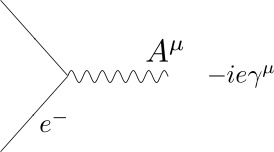
\includegraphics[scale=0.6]{feynmanruleqed} % in feynmanrules.svf as a Layer
  \caption{Feynman rule for QED}
  \label{fig:feynmanruleqed}
\end{figure}
\end{frame}


Para usar esta regla de Feynman debemos aclarar que línea fermiónica corresponde a partícula y cual a antipartícula.
Ver~\ref{fig:feynmanrulesqed}


\begin{frame}[fragile,allowframebreaks]
\begin{figure}
  \centering
  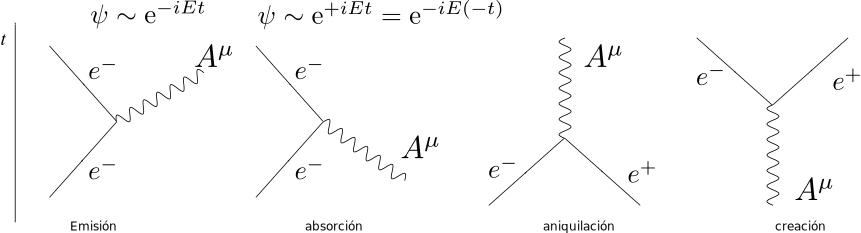
\includegraphics[scale=0.4]{feynmanrulesqed} % in feynmanrules.svf as a Layer
  \caption{Configurations of Feynman rule for QED. The defined positive energy particles (antiparticles) travel in the same (opposite) direction that time. }
  \label{fig:feynmanrulesqed}
\end{figure}
\end{frame}


La repulsión electromagnética esta representada por la figura \ref{fig:qedrepulsion}. En la Figura (a) el primer electrón emite un fotón y se dispersa, mientras que el segundo absorbe el fotón y se dispersa en la dirección opuesta. En la Figura (b) el primer electón absorve el fotón emitido por el segundo electrón. Los dos diagrams se representa por uno único con el fotón en horizontal como se muestra en la Figura (c).

\begin{frame}[fragile,allowframebreaks]
\begin{figure}
  \centering
  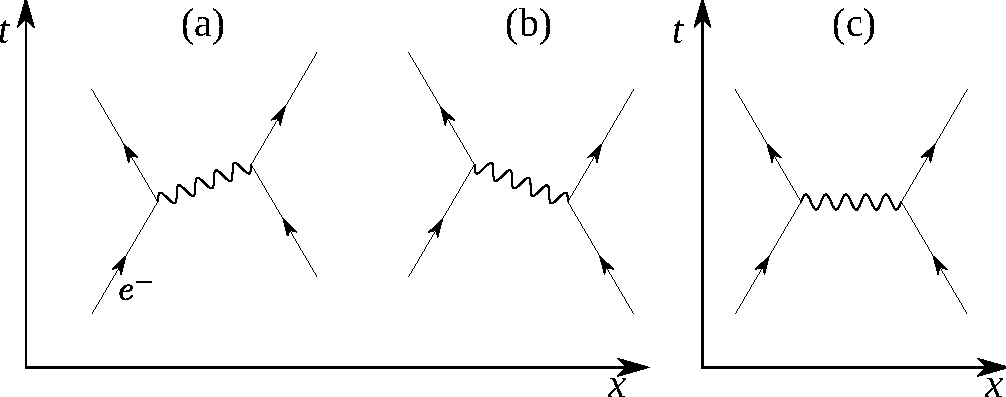
\includegraphics[scale=0.5]{qedrepulsion}
  \caption{Electromagnetic repulsion. The diagrams (a) and (b) are summarized in the diagram (c)}
  \label{fig:qedrepulsion}
\end{figure}
\end{frame}

La aniquilación de un par electrón positrón en un fotones tiene que ser consistente con la conservación de momentum. En general, el cudrimomentum del electron es
\begin{align}
  p^\mu=&(E,\boldsymbol{p}),& \text{such that: }  m^2=p_{\mu}p^{\mu}=& E^2-p^2\,.
\end{align}
mientras que para el fotón es
\begin{align}
  p^\mu=&(E,\boldsymbol{p}),& \text{such that: }  0=p_{\mu}p^{\mu}=& E^2-p^2\,,
\end{align}
y por consiguiente
\begin{align}
  E=|\boldsymbol{p}|\,.
\end{align}

Sin perdida de generalidad, cuando un electrón y su antipartícula, el positrón, sufren una colisión viajando en direcciones opuestas, podemos escoger el sistema de masa, tal que asignando los momentos iniciales como en la figura~\ref{fig:anihilation}
\begin{align}
  \boldsymbol{p}_1-\boldsymbol{p}_{2}=0\,.
\end{align}
La conservación de la cantidad de movimiento garantiza entonces que
\begin{align}
  \boldsymbol{p}'_1-\boldsymbol{p}'_{2}=0\,.
\end{align}
De este modo, si en el estado final hay un sólo fotón, necesariamente este tendría cuadrimomentum nulo, de aquí una Energía nula  en clara violación de la conservación de energía. Por lo tanto, la aniquilación de un electrón y un positrón en radiación electrómagnética, debe dar lugar a aal menos dos fotones, como se muestra en la figura

\begin{frame}[fragile,allowframebreaks]
\begin{figure}
  \centering
  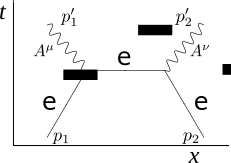
\includegraphics[scale=0.8]{anihilation}
  \caption{Momentum conservation force  annihilation into two photons}
  \label{fig:anihilation}
\end{figure}
\end{frame}

Cada nuevo vértice en un proceso contribuye con un factor $e^{2}$ pues el cálculo de las probabilidades en mecánica cuántica involucran un módulo cuadrado. La cantidad adimensional asociada es la constante de estructura fina
\begin{align}
  \alpha=\frac{e^2}{4\pi}\approx \frac{1}{137}\,.
\end{align}

En el átomo de Hidrógeno, las interacciones electromagnética que mantienen el átomo ligado provienen de la emisión de un fotón por parte del electrón que es absorbido por el protón (y viceversa). Sin embargo, es también la probable que el fotón sea reabsorbido por el propio electrón como se indica en la figura~\ref{fig:selfenergy}. Sin embargo, débido a los dos vérices adicionales, la probabilidad de que esto suceda está suprimida por un factor de $\mathcal{O}({\alpha}^{2})\sim 10^{-3}$. Coloquialmente, esto implicaría que por cada mil fotones que el electrón intercambio con el protón, el propio electrón reaborve uno de ellos. Esto genera un nivel hiperfino en el átomo de hidrógeno con consecuencias medibles experimentalmente. 

\begin{frame}[fragile,allowframebreaks]
\begin{figure}
  \centering
  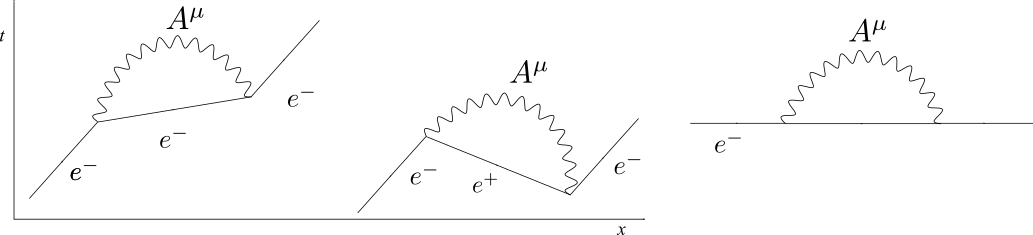
\includegraphics[scale=0.5]{oneloopqed}
  \caption{Electron self-energy}
  \label{fig:selfenergy}
\end{figure}
\end{frame}

Similarmente el fotón puede ``fluctuar con el vacío'', como se muestra la figura~\ref{fig:polarization}

\begin{frame}[fragile,allowframebreaks]

\begin{figure}
  \centering
  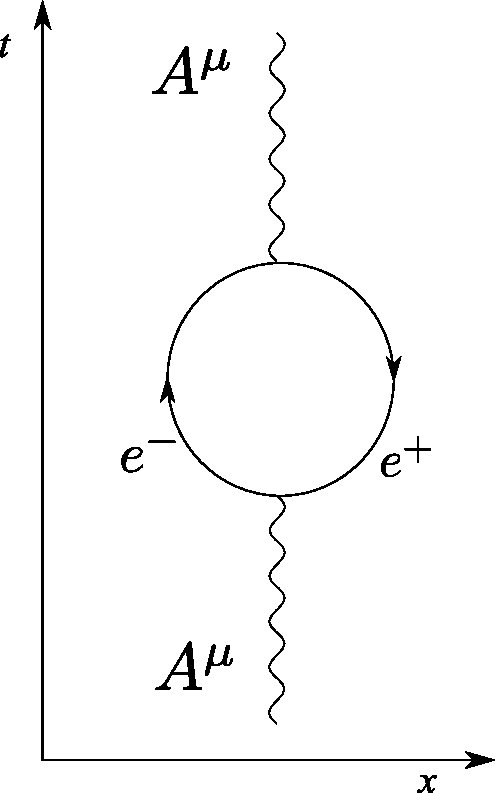
\includegraphics[scale=0.4]{polarization}
  \caption{Vacuum polarization}
  \label{fig:polarization}
\end{figure}
\end{frame}

\textbf{Ejercicio}:
Realize correcciones a un loop a la interacción entre dos electrones de la figura~\ref{fig:qedrepulsion}, incluyendo la demominada \emph{corrección al vérice}.

\section{Momento magnético del electrón}
La correspondiente a la ecuación de Euler-Lagrange para el campo $\overline{\psi}$,
%%%Establecer la ecuación
El Hamiltoniano para el campo electrónico completo en presencia de un campo electromagnética en la QED es
%%expresión para H

\begin{frame}[fragile,allowframebreaks]
El límite no relativista de dicho Hamiltoniano es obtenido en la Apéndice~\ref{sec:limite-no-relat}. El resultado es

\begin{align}
  \widehat{H}\psi
  &=\left[\frac{1}{2m}(i\boldsymbol{\nabla}+q \mathbf{A})^2+q A_0-\left(\frac{q\boldsymbol{\sigma}}{2m}\right)\cdot\mathbf{B}\right]\psi\,.
\end{align}

\end{frame}
En ausencia del campo electromagn\'etico recupermos la Ecuaci\'on de Scrh\"onger para una part\'\i cula libre como era de esperarse. Sin el \'ultimo t\'ermino $({q\boldsymbol{\sigma}}/{2m})\cdot\mathbf{B}$, ser\'\i a el Hamiltoniano de Scr\"odinger para una part\'\i cula cargada en presencia de un campo electromagn\'etico. El t\'ermino adicional es interpretado como la energ\'\i a en un campo magn\'etico, de un momento magn\'etico intr\'\i nseco asociado con un part\'\i cula de Dirac.

\begin{frame}[fragile,allowframebreaks]
Definimos entonces el momento magn\'etico intr\'\i nseco como ($q=-e$)
\begin{align}
  \boldsymbol{\mu}_e&=-\frac{e\boldsymbol{\sigma}}{2m}\nonumber\\
  &=-2\left(\frac{e}{2m}\right)\frac{\boldsymbol{\sigma}}{2}\nonumber\\
  &=-2\left(\frac{e\hbar}{2m}\right)\frac{\boldsymbol{\sigma}}{2}\nonumber\\
  &=-g_e\left(\frac{e\hbar}{2m}\right)\frac{\boldsymbol{\sigma}}{2}\nonumber\\
\end{align}
donde hemos recuperado el factor $\hbar$ y definido el \emph{factor--g} \cite{spin},  $g_e=2$. Se define el momento magn\'etico an\'omalo del electr\'on como
%See https://en.wikipedia.org/wiki/Anomalous_magnetic_dipole_moment
\begin{equation}
  a_e=\frac{g_e-2}{2}
\end{equation}
de modo que $a_e=0$. Sin embargo experimentalmente $a_e\sim10^{-3}$
\begin{equation}
  a_e=0.001\;159\;652\;1859(38)
\end{equation}
\end{frame}
Despu\'es de la segunda cuantizaci\'on, se pueden realizar correcciones perturbativas al valor calculado anteriormente de $g_e$. Dicho c\'alculo ha sido realizado a cuarto orden en teor\'\i a de perturbaciones coincidiendo con el valor experimental hasta la d\'ecima cifra significativa. Este tipo de comprobaciones entre teor\'\i a y experimento ha llevado a considerar la Electrodin\'amica Cu\'antica (QCD) como la mejor teor\'\i a que se halla construido para describir la naturaleza.

\begin{frame}[fragile,allowframebreaks]
Algunas de las cientos de miles de contribuciones, se ilustran en la figura~\ref{fig:5loop}, tomada de la referencia~\cite{Aoyama:2019ryr}
\begin{figure}
  \centering
  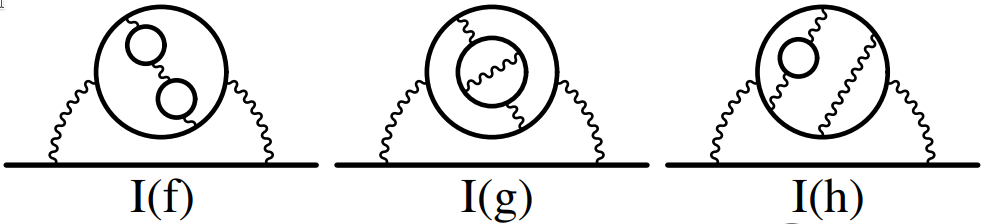
\includegraphics{5loop}
  \caption{Some five-loop correction from~\cite{Aoyama:2019ryr}}
  \label{fig:5loop}
\end{figure}
\end{frame}

\subsection{Paridad}
\begin{frame}[fragile,allowframebreaks]
\begin{align}
  \overline{\psi}\gamma^{\mu}\psi A_{\mu}=&
\xi^{\dagger}\overline{\sigma}^{\mu}\xi A_{\mu}+\eta\sigma^{\mu}\eta^{\dagger} A_{\mu}\nonumber\\
=&(e_L)^{\dagger}\overline{\sigma}^{\mu}e_L A_{\mu}+(e_R)^{\dagger}\sigma^{\mu}e_{R} A_{\mu}\,,
\end{align}
de modo que el fotón se acopla por igual a los campos izquierdos que a los derechos. El Lagrangiano de la QED en términos de espinores de Weyl es:
\begin{align}
  \mathcal{L}=&i(e_L)^{\dagger}\overline{\sigma}^{\mu}\partial_{\mu}e_L A_{\mu}+i(e_R)^{\dagger}\sigma^{\mu}\partial_{\mu}e_{R}
-m \left[ \left( e_R \right)^\dagger e_L+\left( e_L \right)^{\dagger}e_R \right] -\tfrac{1}{4}F^{\mu\nu}F_{\mu\nu}\nonumber\\
   &+eQ \left[(e_L)^{\dagger}\overline{\sigma}^{\mu}e_L+(e_R)^{\dagger}\sigma^{\mu}e_{R}  \right] A_{\mu}
\end{align}
\end{frame}
Se dice entonces que la corriente  electromagnética conserva paridad, es decir es invariante bajo el cambio $L\leftrightarrow R$. 
Una demostración de esta invarianza se muestra en el Apéndice \ref{sec:ferm-quir-de}
%Intentando obtener el operador Hamiltoniano y demás:
%  \begin{align}
%   T^\mu_\nu=&\frac{\partial\mathcal{L}}{\partial\left(\partial_\mu\psi\right)}\partial_\nu\psi+\partial_\nu\bar{\psi}\frac{\partial\mathcal{L}}{\partial\left(\partial_\mu\bar{\psi}\right)}-\mathcal{L}\delta^\mu_\nu\nonumber\\
%   =&i\bar{\psi}\gamma^\mu\partial_\nu\psi-\mathcal{L}\delta^\mu_\nu\,.
% \end{align}
% La expresión para $T^0_i$ es la misma que antes
% \begin{align}
%   T^0_0=i\psi^\dagger\partial_0\psi-i\psi^\dagger\partial_0\psi-i\psi^\dagger\gamma^0\gamma^i\partial_i\psi+m\psi^\dagger\psi-eQ\bar{\psi}\gamma^\mu\psi A_\mu +\tfrac{1}{4}F^{\mu\nu}F_{\mu\nu}.
% \end{align}

%En adelante escribiremos el término sólo para el fermión izquierdo $\psi$ (y el correspondiente antifermion derecho $\psi^{\dagger}$)

\section{Cromodinámica Cuántica}
\label{sec:inter-fuert}

Como se ilustra en la figura~\ref{fig:crosssection}, en cromodinámica cuántica existe la posibilidad que un electrón y un positrón se aniquilen mutuamente en pura energía llevada por un fotón virtual el cual se debe materializar en un par partícula-antipartícula de acuerdo a la energía disponible. Este es el principio de funcionamiento de los aceleradores electrón-positrón donde se generan dos rayos muy energéticos de electrones y positrones los cuales se hacen colisionar en un punto alrededor de un detector de partículas. El detector esta diseñado para reconstruir los productos de la aniquilación del par electrón positrón. Por ejemplo, si el par electrón-positrón colisiona con una energía superior a $\SI{212}{MeV}$, existe la probabilidad que se cree un par muón ($\mu^-$) antimuón $\mu^{+}$. En teoría cuántica de campos de campos a dicho proceso se le llama sección eficaz y se denota como
\begin{frame}[fragile,allowframebreaks]
\begin{align}
  \sigma(e^+\;e^-\rightarrow \mu^+\;\mu^-)
\end{align}

\begin{figure}
  \centering
  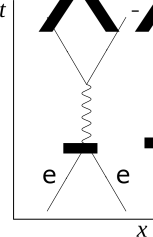
\includegraphics[scale=0.6]{crosssection}
  \caption{Diagrama de Feynman para la aniquilación electrón-positron y la subsecuente creación de un par partícula-antipartícula de acuerdo a la energía disponible}
  \label{fig:crosssection}
\end{figure}
\end{frame}
Aunque el cálculo de dicho proceso está fuera del alcance de una descripción clásica de los campos, dicha probabilidad debe ser proporcional al cuadrado de la carga eléctrica de la partícula producida, en este caso $Q_{\mu}^2=1$, en unidades de la carga del electrón. El conjunto fermiones elementales que interaccionan sólo de forma electrodébil se conoce como \emph{leptones} y esta especificado en la tabla~\ref{tab:leptons}
\begin{frame}
\begin{figure}
  \centering
  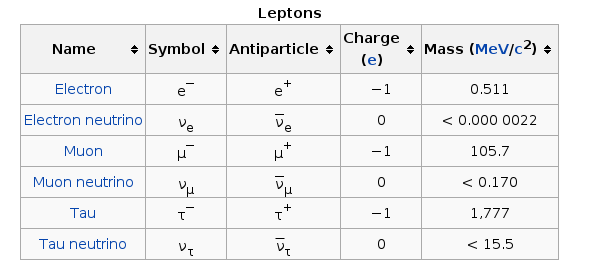
\includegraphics[scale=0.85]{leptons}
  \caption{Leptones de: \url{http://en.wikipedia.org/wiki/List_of_particles}}
  \label{tab:leptons}
\end{figure}
\end{frame}

Con el avance de la tecnología de aceleradores, en la década de los 50 y 60 del siglo pasado se logró establecer la existencia de un zoológico de nuevas partículas, la mayoría de ellas correspondientes a \emph{hadrónes} en el proceso:
\begin{align}
  \sigma(e^+\;e^-\rightarrow \text{hadrónes})\,.
\end{align}
Los protones, neutrones, piones, kaones y demás hadrones, son partículas compuestas de constituyentes elementales llamados quarks. Por ejemplo los protones, neutrones y piones están constituidos de quarks up y down. Los hadrones están dividos en  bariones, $B$, constituidos de tres quarks, y los mesones, $M$, de dos. Para satisfacer el principio de exclusión de Pauli, y justificar el confinamiento de los hadrones, se requiere que cada quark contenga $N_c$ cargas diferentes, llamadas cargas de color, de manera que la carga de color de un hadrón sea cero, de forma similar a como la carga eléctrica de un átomo es cero a pesar de que sus constituyentes poseen carga eléctrica. Muchos resultados experimentales respaldan la existencia de tres cargas de color para cada quark, $N_c=3$. De este modo cada quark $q=u,d,c,s,t,b$, con las propiedades mostradas en la tabla~\ref{tab:quarks}, viene en tres colores
\begin{equation}
  q_\alpha=q_1,q_2,q_3=q_r,q_b,q_g,
\end{equation}
donde los últimos subíndices hacen referencia a los colores red, blue, green. De este modo los Bariones y mesones están descritos por combinaciones singletes de color del tipo $q_r q_b q_g$ y $q_r\bar{q}_r$,
\begin{equation}
\label{eq:199qft}
  B=\frac{1}{\sqrt{6}}\epsilon_{\alpha\beta\gamma}
  \left|q_\alpha q_\beta q_\gamma\right\rangle \qquad M=\frac{1}{\sqrt{3}}\delta^{\alpha\beta}\left|\bar{q}_{\alpha}q_\beta\right\rangle
\end{equation}
Estos estados son singletes de color. Algunos ejemplos de baryones y mesones formados por quarks $u$ y $d$ se muestran en la tabla~\ref{tab:baryonsmesons}

%Comentar sobre la relación Quimica con electrones de Valencia y Física Nuclear con quarks de Valencia

\begin{frame}
\begin{figure}
  \centering
  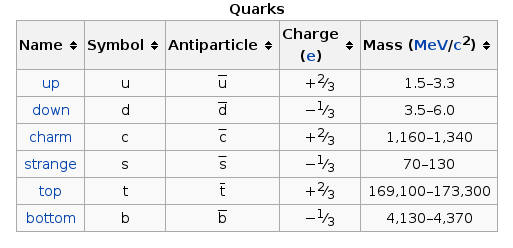
\includegraphics[scale=0.85]{quarks}
  \caption{Quarks de: \url{http://en.wikipedia.org/wiki/List_of_particles}}
  \label{tab:quarks}
\end{figure}
\end{frame}
\begin{frame}[fragile,allowframebreaks]
\begin{figure}
  \centering
  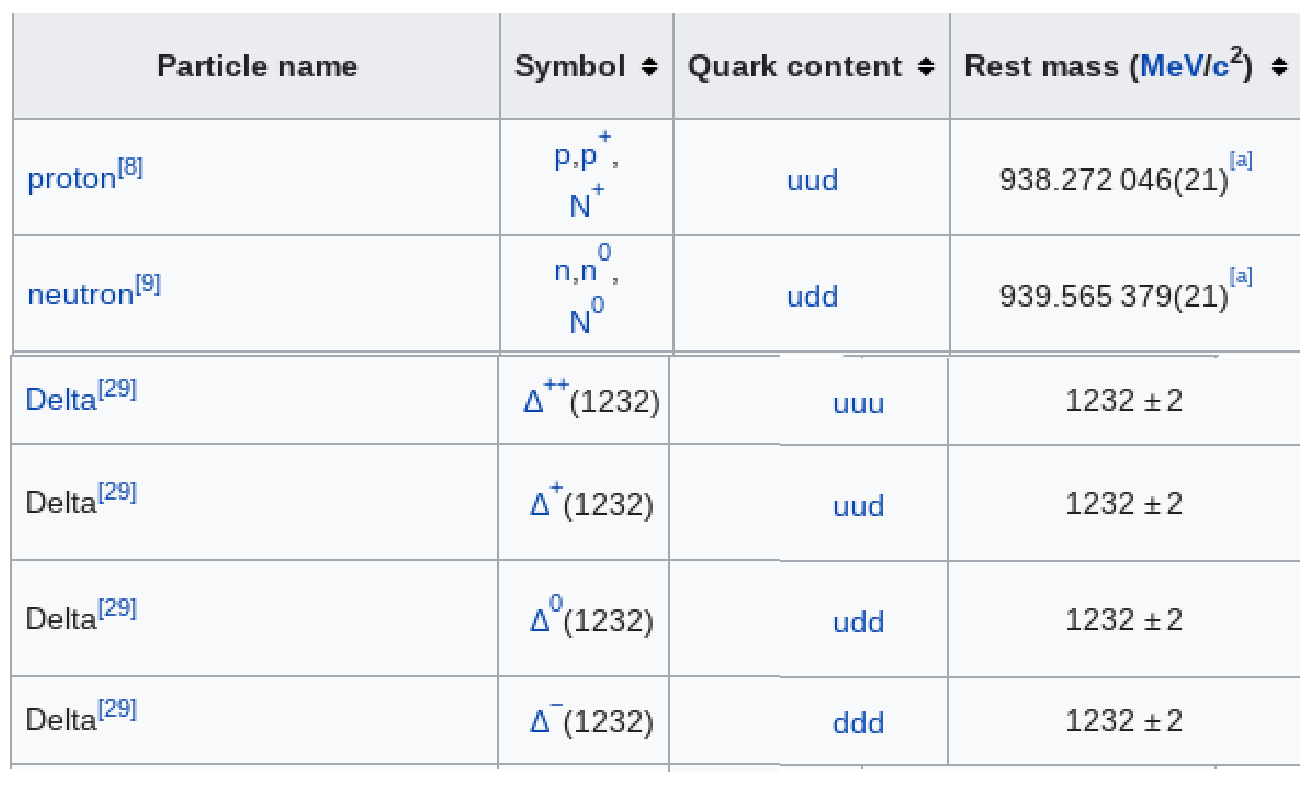
\includegraphics[scale=0.55]{baryons}
  
  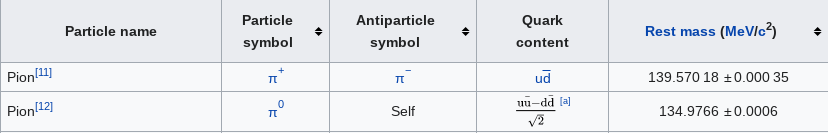
\includegraphics[scale=0.55]{pions}
  \caption{Algunos bariones y mesones de la primera generación de quarks}
  \label{tab:baryonsmesons}
\end{figure}

Una lista completa de bariones está en: \url{https://en.wikipedia.org/wiki/List_of_baryons}\footnote{\url{http://pdg.lbl.gov/2019/tables/contents_tables_baryons.html}}

Una lista completa de mesones está en: \url{https://en.wikipedia.org/wiki/List_of_mesons}\footnote{\url{http://pdg.lbl.gov/2019/tables/contents_tables_mesons.html}}


\end{frame}





Una de las determinaciones de $N_c$ proviene del observable
\begin{align}
  R=&\frac{\sigma(e^+e^-\to\text{hadrones})}{\sigma(e^+e^-\to\mu^+\mu^-)}
\end{align}

Para $f=u,d,s,c,b,t$, (en orden de masa) tenemos que para una energía donde se pueden producir hadrones compuestos de hasta  quarks $f_{\text{max}}$
\begin{align}
  R\approx&\frac{\sum_{f=u}^{f_{\text{max}}}\sum_{\alpha=1}^{N_c}\sigma(e^+e^-\to f_\alpha\bar{f}_\alpha)}{\sigma(e^+e^-\to\mu^+\mu^-)}\nonumber\\
  R\approx&N_c\frac{\sum_{f=u}^{f_{\text{max}}}\sigma(e^+e^-\to f\bar{f})}{\sigma(e^+e^-\to\mu^+\mu^-)}
\end{align}
De este modo $R$ esta dado por la suma de las cargas eléctricas al cuadrado
\begin{align}
\label{eq:254qft}
R\approx&N_c\frac{\sum_f Q_f^2}{Q_\mu^2}\nonumber\\
=
&N_c\sum_{f=u}^{f_{\text{max}}} Q_f^2\nonumber\\
=&
\begin{cases}
  N_c[(\frac{2}{3})^2+2(\frac{-1}{3})^2]=\frac{2}{3}N_c&f=u,d,s,\;f_{\text{max}}=s\\
  N_c[2(\frac{2}{3})^2+2(\frac{-1}{3})^2]=\frac{10}{9}N_c&f_{\text{max}}=c\\
  N_c[2(\frac{2}{3})^2+3(\frac{-1}{3})^2]=\frac{11}{9}N_c&f_{\text{max}}=b
\end{cases}\nonumber\\
=&
\begin{cases}
  2&N_c=3,\qquad f_{\text{max}}=s\\
  \frac{10}{3}&N_c=3,\qquad f_{\text{max}}=c\\
  \frac{11}{3}&N_c=3,\qquad f_{\text{max}}=b\\
\end{cases}
\end{align}
%\left(\right)
En la figura, tomada de \cite{a}, se muestra el gráfico de $R$ con respecto a $\sqrt{s}$ (la energía de centro de masa de la colisión). Se observan dos escalones, uno que va hasta una energía $\sqrt{s}\approx4\,$GeV que corresponden a $f=u,d,s$, con un $R\approx2$,  y otro hasta $\sqrt{s}\approx40\,$GeV que corresponde a $f=u,d,s,c,b$, con un $R\approx3.7\approx11/3$. Los dos valores de $R$ son compatibles con los esperados de la ec.~\eqref{eq:254qft}. Como referencia también se señalan los valores para $N_c=4$ (en rojo). 
\begin{frame}
\begin{figure}
  \centering
  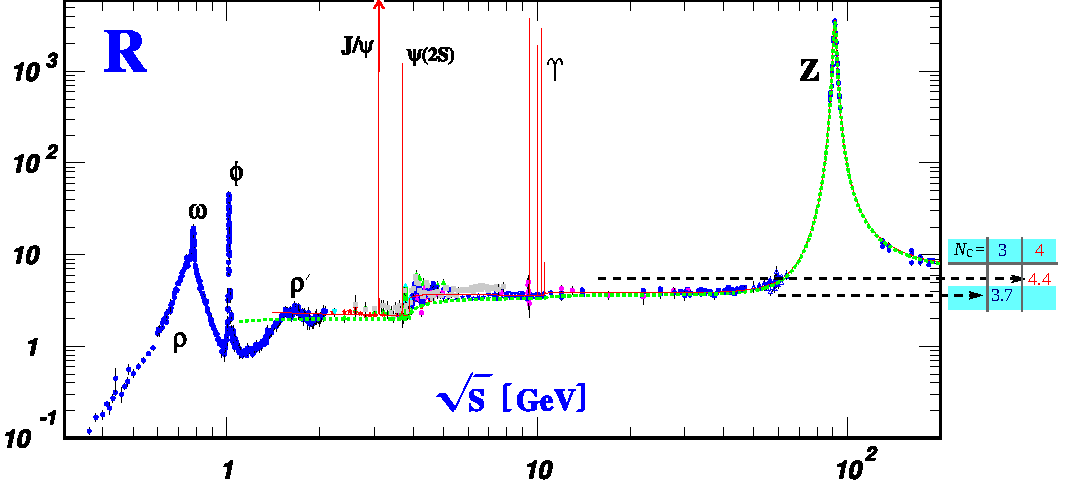
\includegraphics[scale=0.65]{r}
  \caption{Datos para $R$}
  \label{fig:r}
\end{figure}
\end{frame}

%Comentar sobre Babar (ver Miro Notebook)


Si queremos que el color sea una carga conservada como la carga eléctrica, ésta debe ser la consecuencia de una simetría gauge local. Para tener tres cargas diferentes la posibilidad más simple es imponer la simetría $SU(3)_c$, tal que tengamos un vector compuesto de 3 espinores de Dirac en el espacio de color:

\begin{frame}  
\begin{equation}
  \Psi=
  \begin{pmatrix}
    \psi_r\\
    \psi_b\\
    \psi_g
  \end{pmatrix}
  =
  \begin{pmatrix}
    q_r\\
    q_b\\
    q_g
  \end{pmatrix}\qquad q=u,d,c,s,t,b\,.
\end{equation}
\end{frame}
El Lagrangiano de Dirac con invarianza gauge global $SU(3)$, para un quark, se puede escribir como
\begin{equation}
  \label{eq:128qft}
  \mathcal{L}_{\text{global}}=i\bar{\Psi}\gamma^\mu\partial_\mu\Psi-m\bar{\Psi}\Psi,
\end{equation}
El análisis es completamente simiar si se usa el Lagrangiano sólo para los fermiones de Weyl izquierdos
\begin{align}
    \mathcal{L}_{\text{global}}=i\bar{\Psi}\overline{\sigma}^\mu\partial_\mu\Psi
\end{align}

\begin{frame}
  
La transformación gauge local bajo $SU(3)$ es
\begin{equation}
  \Psi\to \Psi'=\exp\left(i\theta_a(x)\frac{\lambda^a}{2}\right)\Psi.
\end{equation}
donde $a=1,\ldots,8$, $\lambda_a/2$ son los ocho generadores de $SU(3)$ y $\theta_a(x)$ son los parámetros de la transformación global. Los generadores de $SU(3)$
\begin{align}
  \Lambda^a\equiv\frac{\lambda^a}{2}\,,
\end{align}
satisfacen el álgebra
\begin{equation}
  \left[\frac{\lambda^a}{2},\frac{\lambda^b}{2}\right]=if^{abc}\frac{\lambda^c}{2}\,,
\end{equation}
donde $f^{abc}$ son las constantes de estructura fina de $SU(3)$.
\end{frame}

Las ocho matrices $3\times3$ $\lambda^a$ se pueden construir a partir de las tres matrices de Pauli, pero su forma explícita no es necesaria en la siguiente discusión.

En un análisis similar al de la sección \ref{sec:diracs-lagrangian} tenemos que la Acción invariante gauge local bajo $SU(3)_c$, se obtiene de reemplazar la derivada normal por la derivada covariante. Para compensar los 8 cambios asociados a los 8 parámetros $\theta_a(x)$, la derivada covariante debe definirse en términos de 8 campos vectoriales $G^\nu_a$, que llamaremos campos de gluones
\begin{frame}[fragile,allowframebreaks]
\begin{equation}
  \label{eq:127qft}
  \mathcal{L}_{\text{local}}=i\bar{\Psi}\gamma^\mu\mathcal{D}_\mu\Psi-m\bar{\Psi}\Psi
  -\mathcal{L}\left( G^{\nu}_{a},\partial_{\mu}G^{\nu}_{a} \right)\,.%\frac{1}{2}\operatorname{Tr}\left({G}^{\mu\nu}{G}_{\mu\nu}\right),
\end{equation}
donde
\begin{align}
  \label{eq:qcdtr}
  \Psi\to \Psi'&=U(x)\Psi\nonumber\\
  \mathcal{D}_\mu\Psi\to \left(\mathcal{D}_\mu\Psi\right)'&
  =U(x)\mathcal{D}_\mu\Psi,
\end{align}
con la matriz $3\times 3$
\begin{align}
  U(x)=\exp\left[i\theta_a(x){\Lambda^a}\right]\,,
\end{align}
y
\begin{equation}
  \mathcal{D}_\mu=\partial_\mu-i g_s{\Lambda_a}G_\mu^a\equiv\partial_\mu-i g_s {G}_\mu
\end{equation}
donde hemos definido la matriz $3\times 3$  $G_\mu$, como
\begin{equation}
  \left({G}_\mu\right)_{\alpha\beta}=\left( \Lambda_a \right)_{\alpha\beta}G_\mu^a
\end{equation}
\end{frame}
Este Lagrangiano da lugar a la interacción fuerte y es llamado el Lagrangiano de la Cromodinámica Cuántica, o el Lagrangiano de la QCD de sus siglas en Inglés.

De \eqref{eq:qcdtr}, tenemos
\begin{align}
   \mathcal{D}_\mu\Psi\to \left(\mathcal{D}_\mu\Psi\right)'=&\mathcal{D}'_\mu\Psi'
  =U(x)\mathcal{D}_\mu\Psi\nonumber\\
\mathcal{D}'_\mu U\Psi
  =U(x)\mathcal{D}_\mu\Psi\,.
\end{align}
Por consiguiente
\begin{equation}
  {\mathcal{D}'}^\mu U=U\mathcal{D}^\mu
\end{equation}
\begin{equation}
  \mathcal{D}^\mu\to\left(
    \mathcal{D}^\mu
  \right)'=U\mathcal{D}^\mu U^{-1}
\end{equation}
Desarrollando a ambos lados
\begin{align}
  \label{eq:251qft}
   {\mathcal{D}}^\mu\psi\to{\left({\mathcal{D}}^\mu\psi\right)}'=
  {\mathcal{D}^\mu}'\psi'=&{\mathcal{D}^\mu}'\psi'\nonumber\\
  (\partial^\mu-i g_s {G'}^\mu) U\psi=&U\mathcal{D}^\mu U^{-1}U\psi\nonumber\\
  (\partial^\mu-i g_s {G'}^\mu) U\psi=&U(\partial^\mu-i g_s {G}^\mu)\psi\nonumber\\
  U\partial^\mu\psi+(\partial^\mu U)\psi-i g_s {G'}^\mu U \psi=&U\partial^\mu\phi-i g_s U {G}^\mu \psi\nonumber\\
  (\partial^\mu U)\psi-i g_s {G'}^\mu U \psi=&-i g_s U {G}^\mu \psi\nonumber\\
  -i g_s {G'}^\mu U \psi=&-(\partial^\mu U)\psi-i g_s U {G}^\mu \psi\,,
\end{align}
de modo que
\begin{align}
 G^{\mu}\to     {G'}^\mu U =&\frac{1}{i g_s}(\partial^\mu U)+ U{G}^\mu \nonumber\\
 G^{\mu}\to  {G'}^\mu  =&-\frac{i}{g_s}(\partial^\mu U)U^{-1}+ U{G}^\mu U^{-1}\,.
\end{align}

Como $U$ es unitaria, la transformación de los campos gauge puede escribirse como
\begin{equation}
    {G}^\mu\to\left({G}^\mu\right)'=U{G}^\mu U^{\dagger}-\frac{i}{g_s}\left(\partial^\mu U\right)U^\dagger.
\end{equation}
Como
\begin{align}
  \partial^{\mu}U= \partial^{\mu}\exp\left[i\theta_a(x){\Lambda^a}\right]
  = \left( \partial^{\mu}i\theta_a(x)\right){\Lambda^a}\exp\left[i\theta_a(x){\Lambda^a}\right]
   = \left( \partial^{\mu}i\theta_a(x)\right){\Lambda^a}U\,,
\end{align}
entonces
\begin{frame}[fragile,allowframebreaks]
\begin{align}
   {G}^\mu\to\left({G}^\mu\right)'=U{G}^\mu U^{\dagger}+\frac{1}{g_s}{\Lambda^a} \partial^{\mu}\theta_a(x)\,.
\end{align}
y la expresión en ec.~\eqref{eq:gnrlaggtr} en efecto es suficiente general y para $\operatorname{SU}(3)$ queda
\begin{align}
   \Lambda^a{G'}^\mu_a=&U\Lambda^cG^\mu_cU-\frac{1}{g_s}\Lambda^e(\partial^\mu\theta_e)\,.
\end{align}
Entonces, haciendo la expansión a primer orden en $\theta_{a}(x)$ de $U$
\begin{align}
\label{eq:Gmuinv}
  \Lambda^a{G'}^\mu_a\approx&(1+i\theta_b\Lambda^b)\Lambda^cG^\mu_c(1-i\theta_d\Lambda^d)+\frac{1}{g_s}\Lambda^e\partial^\mu\theta_e\nonumber\\
  =&(\Lambda^c+i\theta_b\Lambda^b\Lambda^c)(1-i\theta_d\Lambda^d)G^\mu_c+\frac{1}{g_s}\Lambda^e\partial^\mu\theta_e\nonumber\\
  \approx&[\Lambda^c-i\theta_d\Lambda^c\Lambda^d+i\theta_b\Lambda^b\Lambda^c]G^\mu_c+\frac{1}{g_s}\Lambda^e\partial^\mu\theta_e\nonumber\\
  =&[\Lambda^c-i\theta_b(\Lambda^c\Lambda^b-\Lambda^b\Lambda^c)]G^\mu_c+\frac{1}{g_s}\Lambda^e\partial^\mu\theta_e\nonumber\\
  =&\Lambda^aG^\mu_a-i(i f^{acb}\Lambda^a)G^\mu_c\theta_b+\frac{1}{g_s}\Lambda^a\partial^\mu\theta_a\nonumber\\
  =&\Lambda^a\left(G^\mu_a+\frac{1}{g_s}\partial^\mu\theta_a+f^{acb}G^\mu_c\theta_b\right),
\end{align}
de donde
\begin{align}
  \label{eq:gmutrinf}
  G^\mu_a\to {G'}^\mu_a\approx&G^\mu_a+\frac{1}{g_s}\partial^\mu\theta_a+{f_a}^{bc}G^\mu_b\theta_c\,,
\end{align}
que se reduce al caso Abeliano cuando las constates de estructura son cero. Como era de esperarse cada campo gauge tiene asociado un parámetro de transformación gauge $\theta_a(x)$.
\end{frame}

\begin{frame}[fragile,allowframebreaks]
  \begin{table}
    \centering
    \small
    \begin{tabular}{l|l|l}
      QED & QCD & Diferencia\\\hline
$      \overline{\psi}\left(i\gamma^\mu\mathcal{D}_\mu-m\right)\psi +\mathcal{L} \left(A_{\nu},\partial A_{\nu}  \right)$ & $      \overline{\Psi}\left(i\gamma^\mu\mathcal{D}_\mu-m\right)\Psi +\mathcal{L} \left(G_{\nu},\partial G_{\nu}  \right)$ & $1\times 1 \to 3\times 3$: ($\mathcal{D}_{\mu}$)\\ 
$\mathcal{D}_{\mu}=\partial_{\mu}-i e A_{\mu}$ & $\mathcal{D}_{\mu}=\partial_{\mu}-i g_s G_{\mu}$ & $1\times 1 \to 3\times 3$: ($A_{\mu}\to G_{\mu}$)\\ 
$A_{\mu}\to \widehat{Q}A_{\mu}$ & $G_{\mu}=\Lambda_{a} G_{\mu}^{a}$,\qquad $a=1,\cdots,8$ & $1\times 1 \to 3\times 3$: ($\widehat{Q}\to\Lambda_{a}$)\\ 
$A_{\mu}$&$ G_{\mu}^1,\cdots ,G_{\mu}^8$& $1\to 8$ (Gauge fields)\\
$    {A}^\mu\to {A}^{\prime\mu}=U{A}^\mu U^{*}-\frac{i}{e}\left(\partial^\mu U\right)U^*$&
$ {G}^\mu\to {G}^{\prime\mu}=U{G}^\mu U^{\dagger}-\frac{i}{g_s}\left(\partial^\mu U\right)U^\dagger$
&$1\times 1 \to 3\times 3$: ($U$)\\ 
$U=\exp(i\widehat{Q}\theta)$ & $U=\exp(i\Lambda_{a}\theta^{a})$& $1\to 8$: ($\theta\to\theta_{1},\cdots,\theta_{8}$) \\
      $A^\mu\to {A'}^\mu_a\approx A^\mu+\frac{1}{e}\partial^\mu\theta$ &
$G^\mu_a\to {G'}^\mu_a\approx G^\mu_a+\frac{1}{g_s}\partial^\mu\theta_a+{f_a}^{bc}G^\mu_b\theta_c$ &\parbox{3.5cm}{radiación $\to$ ra\-dia\-ción\--ma\-teria}  \\
$\alpha=\dfrac{e^2}{4\pi}\approx 1/137$ & $\alpha_s=\dfrac{g_s^2}{4\pi}>1$ & \parbox{3.5cm}{perturbativa $\to$ no per\-tur\-ba\-ti\-va}  \\
    \end{tabular}
    \caption{Comparación entre la QED y la QCD}
  \end{table}
\end{frame}


\subsection{Tensores cromodinámicos}

%Logica actual:
% 1 G es campo de materia y requiere definir una derivada covariante
% 2 Construya tensor con derivadas covariantes
% 3 Encuentre como tranforma un tensor
% 2 Demuestre que la derivada covariante de Gmunu transforma como Gmunu


Note entonces que en el lenguage de los teoremas de Noether, el campo $G^{\mu}_{a}$ transforma como un campo material y un campo de radiación a la vez, es decir, su transformación depende tanto del parámetro como de la derivada del parámetro. Por consiguiente, es conveniente definir la derivada covariante del campo $G^{\nu}_{a}$. Para ello se debe introducir la representación adjunta de $\operatorname{SU}(N)$.

\begin{frame}[fragile,allowframebreaks]
La representación adjunta de $\operatorname{SU}(3)$, consiste en las 8 matrices $8\times 8$
\begin{align}
  \left[  \widetilde{\Lambda}^{a}\right]_{bc}=-i {f^{a}}_{bc}\,.
\end{align}
\end{frame}

\noindent
\textbf{Ejemplo:} Definiendo $\Sigma_i$ como las matrices $3\times3$ generadores de $\operatorname{SU}(2)$ en la representaci\'on adjunta
\begin{align}
  (\Sigma_i)_{jk}=-i\epsilon_{ijk}\,,
\end{align}
hemos comprobado en la ec.~\eqref{eq:adjrepsu2} que
\begin{align}
  \left[{\Sigma_i},{\Sigma_j}\right]&=i\epsilon_{ijk}{\Sigma_k}\nonumber\\
  \left[{\Sigma_i},{\Sigma_j}\right]_{lm}&=i\epsilon_{ijk}(\Sigma_k)_{lm}\,.
\end{align}
\noindent
\textbf{Ejercicio:} Demostar que la representación adjunta satisface el álgebra de $\operatorname{SU}(3)$.

\begin{frame}[fragile,allowframebreaks]
La derivada covariante en la representación adjunta es
\begin{align}
  \mathcal{D}_{\mu}=&\mathbf{1}\partial_{\mu}-i g_s \mathbb{G}_{\mu}  \nonumber\\
=&\mathbf{1}\partial_{\mu}-i g_s \widetilde{\Lambda}_a G_{\mu}^{a} \,,
\end{align}
donde
\begin{align}
  \mathbb{G}_{\mu}\equiv \widetilde{\Lambda}_a G_{\mu}^{a}\,,
\end{align}
\end{frame}
es ahora una matriz $8\times8$ de campos de gluones en la representación adjunta. En componentes
\begin{align}
 \left[\mathcal{D}_{\mu} \right]^b_c=&\delta^b_c\partial_{\mu}-i g_{s}\left[ \widetilde{\Lambda}_{a} G^a_{\mu} \right]^b_c \nonumber\\
                  =&\delta^b_c\partial_{\mu}- g_{s} {f_{a}}^{bc}  G^a_{\mu} \,.
\end{align}

Esta derivada se puede aplicar a la matriz de campo de gluones:
\begin{align}
  \mathcal{D}_{\mu}  \mathbb{G}_{\nu}=& \left(\mathbf{1}\partial_{\mu}-i g_s \mathbb{G}_{\mu} \right)\mathbb{G}_{\nu}
\end{align}
o en componentes
\begin{align}
  \left[ \mathcal{D}_{\mu} \right]^{a}_{b} \left[ \mathbb{G}_{\nu} \right]^b_c=& \left(\delta^a_b\partial_{\mu}-i g_s \left[ \mathbb{G}_{\mu} \right]^{a}_{b} \right)\left[ \mathbb{G}_{\nu} \right]^b_c \nonumber\\
    =& \left(\delta^a_b\partial_{\mu}-i g_s \left[  \widetilde{\Lambda}_c \right]^a_b G^c_{\mu} \right) \left[  \widetilde{\Lambda}_d \right]^b_cG_{\nu}^{d}\,.
\end{align}

Veamos como transforma la derivada covariante de la matriz de campos de gluones en la representación adjunta, donde un elemento $8\times 8$ del grupo $\operatorname{SU}(3)$ se define ahora como
\begin{align}
  \widetilde{U}=\exp \left[ i\theta_a(x) \widetilde{\Lambda} \right].
\end{align}
Entonces
\begin{align}
\label{eq:tdcg}
 \mathcal{D}_{\mu} \mathbb{G}_{\nu}\to   \left(   \mathcal{D}_{\mu} \mathbb{G}_{\nu} \right)' =&
\left[\boldsymbol{1}\partial_{\mu}-i g_s\left(\widetilde{U} \mathbb{G}_\mu \widetilde{U}^{\dagger}-\frac{i}{g_s}\left(\partial_\mu \widetilde{U}\right)\widetilde{U}^\dagger  \right)   \right] \left(\widetilde{U} \mathbb{G}_\nu \widetilde{U}^{\dagger}-\frac{i}{g_s}\left(\partial_\nu \widetilde{U}\right)\widetilde{U}^\dagger  \right) \nonumber\\
=&
\left[\boldsymbol{1}\partial_{\mu}-i g_s\widetilde{U} \mathbb{G}_\mu \widetilde{U}^{\dagger}-\left(\partial_\mu \widetilde{U}\right)\widetilde{U}^\dagger   \right] \left(\widetilde{U} \mathbb{G}_\nu \widetilde{U}^{\dagger}-\frac{i}{g_s}\left(\partial_\nu \widetilde{U}\right)\widetilde{U}^\dagger  \right) \nonumber\\
=&
\partial_{\mu} \left(\widetilde{U} \mathbb{G}_\nu \widetilde{U}^{\dagger}-\frac{i}{g_s}\left(\partial_\nu \widetilde{U}\right)\widetilde{U}^\dagger  \right)
-i g_s\widetilde{U} \mathbb{G}_\mu \widetilde{U}^{\dagger}\left(\widetilde{U} \mathbb{G}_\nu \widetilde{U}^{\dagger}-\frac{i}{g_s}\left(\partial_\nu \widetilde{U}\right)\widetilde{U}^\dagger  \right)
\nonumber\\
&-\left(\partial_\mu \widetilde{U}\right)\widetilde{U}^\dagger\left(\widetilde{U} \mathbb{G}_\nu \widetilde{U}^{\dagger}-\frac{i}{g_s}\left(\partial_\nu \widetilde{U}\right)\widetilde{U}^\dagger  \right) \nonumber\\
  =& \cancel{\left(\partial_{\mu} \widetilde{U} \right) \mathbb{G}_\nu \widetilde{U}^{\dagger}} + \widetilde{U}
  \left( \partial_{\mu}\mathbb{G}_\nu \right) \widetilde{U}^{\dagger} + \widetilde{U}
  \mathbb{G}_{\nu} \partial_{\mu} \widetilde{U}^{\dagger} -\frac{i}{g_s}\partial_{\mu}
  \left[ \left( \partial_{\nu}\widetilde{U} \right)\widetilde{U}^{\dagger} \right]
  \nonumber\\
  &-i g_s \widetilde{U} \mathbb{G}_{\mu}\mathbb{G}_{\nu}\widetilde{U}^{\dagger}- \widetilde{U}\mathbb{G}_{\mu} \widetilde{U}^{\dagger} \left( \partial_{\nu} \widetilde{U}\right)\widetilde{U}^{\dagger} \nonumber\\
  &-\cancel{\left( \partial_{\mu}\widetilde{U} \right)\mathbb{G}_{\nu} \widetilde{U}^{\dagger}}
  +\frac{i}{g_s} \left( \partial_{\mu}\widetilde{U} \right) \widetilde{U}^{\dagger} \left( \partial_{\nu}\widetilde{U} \right) \widetilde{U}^{\dagger} \nonumber\\
  =& \widetilde{U} \left( \partial_{\mu}\mathbb{G}_\nu \right) \widetilde{U}^{\dagger} + \widetilde{U}
  \mathbb{G}_{\nu} \partial_{\mu} \widetilde{U}^{\dagger}
  -\cancel{\frac{i}{g_s}\partial_{\mu} \left[ \widetilde{U}
      \widetilde{U}^{\dagger}\left( \partial_{\nu}\widetilde{U} \right)\widetilde{U}^{\dagger} \right]}
  \nonumber\\
  &-i g_s \widetilde{U} \mathbb{G}_{\mu}\mathbb{G}_{\nu}\widetilde{U}^{\dagger}- \widetilde{U}\mathbb{G}_{\mu}
  \widetilde{U}^{\dagger}\cancel{ \partial_{\nu}\left( \widetilde{U}\widetilde{U}^{\dagger} \right)}+
  \widetilde{U}\mathbb{G}_{\mu} \widetilde{U}^{\dagger} \widetilde{U}\partial_{\nu}\widetilde{U}^{\dagger}
  \nonumber\\
  &+\cancel{\frac{i}{g_s} \partial_{\mu} \left[ \widetilde{U} \widetilde{U}^{\dagger}
      \left( \partial_{\nu}\widetilde{U} \right) \widetilde{U}^{\dagger}\right]}-
  \frac{i}{g_s} \widetilde{U} \partial_{\mu} \left[ \widetilde{U}^{\dagger}
    \left( \partial_{\nu}\widetilde{U} \right) \widetilde{U}^{\dagger}\right]
\end{align}
Ya que
\begin{align}
 \partial_{\mu} \left[ \widetilde{U}^{\dagger}
    \left( \partial_{\nu}\widetilde{U} \right) \widetilde{U}^{\dagger}\right]=&
 \partial_{\mu} \left[ \widetilde{U}^{\dagger}
    \cancel{\partial_{\nu}\left( \widetilde{U} \widetilde{U}^{\dagger}\right)} -\widetilde{U}^{\dagger}\widetilde{U} \partial_{\nu} \widetilde{U}^{\dagger}\right] \nonumber\\
=&- \partial_{\mu} \left[ \widetilde{U}^{\dagger} \widetilde{U} \partial_{\nu} \widetilde{U}^{\dagger}\right] \nonumber\\
=&- \partial_{\mu}  \partial_{\nu} \widetilde{U}^{\dagger} \,,
\end{align}
entonces
\begin{align}
\label{eq:Dmup}
\mathcal{D}_{\mu} \mathbb{G}_{\nu}\to   \left(   \mathcal{D}_{\mu} \mathbb{G}_{\nu} \right)' =& \widetilde{U} \left[ \left( \partial_{\mu}-ig_s \mathbb{G}_{\mu} \right)\mathbb{G}_\nu   \right]\widetilde{U}^{\dagger}
    + \widetilde{U} \left[ \mathbb{G}_{\nu} \partial_{\mu}+\mathbb{G}_{\mu}\partial_{\nu}+\frac{i}{g_s} \partial_{\mu}\partial_{\nu} \right] \widetilde{U}^{\dagger} \nonumber\\
 =& \widetilde{U} \left( \mathcal{D}_{\mu}\mathbb{G}_\nu   \right)\widetilde{U}^{\dagger}
    + \widetilde{U} \left[ \mathbb{G}_{\nu} \partial_{\mu}+\mathbb{G}_{\mu}\partial_{\nu}+\frac{i}{g_s} \partial_{\mu}\partial_{\nu} \right] \widetilde{U}^{\dagger} \,.%\nonumber\\
 %  =& \widetilde{U} \left( \mathcal{D}_{\mu}\mathbb{G}_\nu   \right)\widetilde{U}^{\dagger}
 %    + \widetilde{U}  \mathbb{G}_{\nu} \partial_{\mu}\widetilde{U}^{\dagger}-\frac{i}{g_s} \widetilde{U}\left(\partial_{\mu}+ig_s \mathbb{G}_{\mu} \right)\partial_{\nu}  \widetilde{U}^{\dagger} \nonumber\\
 % =& \widetilde{U} \left( \mathcal{D}_{\mu}\mathbb{G}_\nu   \right)\widetilde{U}^{\dagger}
 %  \right]  + \widetilde{U}  \mathbb{G}_{\nu} \partial_{\mu} \widetilde{U}^{\dagger}-\frac{i}{g_s}\widetilde{U} \mathcal{D}_{\mu}^{\dagger}\partial_{\nu} \widetilde{U}^{\dagger}  \nonumber\\
\end{align} 
Por consiguiente, la ``derivada covariante'' de la matriz del campo de gluones no transforma como la la matriz del campo de gluones. Una discusión al respecto se puede encontrar en~\cite{2015arXiv151203827R}.

\begin{frame}[fragile,allowframebreaks]
Note que si definimos la matriz de tensores de campos de gluones como
\begin{align}
   \mathbb{G}_{\mu\nu}\equiv & \mathcal{D}_{\mu} \mathbb{G}_{\nu}-\mathcal{D}_{\nu} \mathbb{G}_{\mu} 
\end{align}
entonces,
\begin{align}
   \mathbb{G}_{\mu\nu}\to  \mathbb{G}'_{\mu\nu}=\left( \mathcal{D}_{\mu} \mathbb{G}_{\nu} \right)'-\left( \mathcal{D}_{\nu} \mathbb{G}_{\mu}  \right)'\,,
\end{align}
y usando \eqref{eq:Dmup} da lugar a
\begin{align}
\label{eq:ugum}
    \mathbb{G}_{\mu\nu}\to  \mathbb{G}'_{\mu\nu}=&  \widetilde{U} \left\{ \left( \mathcal{D}_{\mu}\mathbb{G}_\nu   \right)
    +  \left[ \mathbb{G}_{\nu} \partial_{\mu}+\mathbb{G}_{\mu}\partial_{\nu}+\frac{i}{g_s} \partial_{\mu}\partial_{\nu} \right]
  -   \left( \mathcal{D}_{\nu}\mathbb{G}_\mu   \right)
    - \left[ \mathbb{G}_{\mu} \partial_{\nu}-\mathbb{G}_{\nu}\partial_{\mu}-\frac{i}{g_s} \partial_{\nu}\partial_{\mu} \right]  \right\} \widetilde{U}^{\dagger} \nonumber\\
=&  \widetilde{U} \left[  \mathcal{D}_{\mu}\mathbb{G}_\nu 
    -   \mathcal{D}_{\nu}\mathbb{G}_\mu
  \right] \widetilde{U}^{\dagger} \nonumber\\
=& \widetilde{U} \mathbb{G}_{\mu\nu} \widetilde{U}^{\dagger}\,.
\end{align}
Esto es justo lo que se espera de la transformación de un tensor para un grupo de simetría continuo.
\end{frame}

Como hemos visto en el caso electromagnético, para demostrar la invarianza del Lagragiano electromagnético en la ec.~\eqref{eq:invlorff}, es necesario que en efecto el tensor electromagnético transforme como un tensor en el espacio de Lorentz:
\begin{align}
  F_{\mu\nu}(x) \to F'_{\mu\nu}(x)  =& { \Lambda_{\mu}}^{\alpha}F_{\alpha\beta}\left( \Lambda^{-1}x \right)\,
                   {\left( \Lambda^{-1} \right)^{\beta}}_{\nu} \,.
\end{align}


Sin embargo, para el tensor electromagnético la transformación bajo $\operatorname{U}(1)_Q$ es trivial.

Retornado a la definición la matriz de tensores de campos gauge para una teoría no Abeliana $\operatorname{SU}(3)$,
\begin{frame}[fragile,allowframebreaks]
si imponemos que la derivada covariante de $\mathbb{G}_{\mu\nu}$ transforme como $\mathbb{G}_{\mu\nu}$\footnote{o asumiendo simplemente que la propiedas de la derivada covariante no dependen de la representación}
\begin{align}
  \mathcal{D}_{\mu}\mathbb{G}^{\mu\nu} \to \left(  \mathcal{D}_{\mu}\mathbb{G}^{\mu\nu}  \right)'=
    \widetilde{U} \left( \mathcal{D}_{\mu}\mathbb{G}^{\mu\nu} \right)  \widetilde{U}^{\dagger}\,,
\end{align}
entonces
\begin{align}
  \mathcal{D}_{\mu}'\mathbb{G}^{\prime \mu\nu}
  =\widetilde{U}  \mathcal{D}_{\mu}\mathbb{G}^{\mu\nu}  \widetilde{U}^{\dagger}\nonumber\\
  =\widetilde{U} \mathcal{D}_{\mu}\widetilde{U}^{\dagger} \widetilde{U} \mathbb{G}^{\mu\nu}  \widetilde{U}^{\dagger}\nonumber\\
  =\widetilde{U} \mathcal{D}_{\mu}\widetilde{U}^{\dagger}  \mathbb{G}^{\prime \mu\nu}\,,
\end{align}
y obtenemos que
\begin{align}
{\mathcal{D}}^\mu \to   {\mathcal{D}'}^\mu =\widetilde{U} {\mathcal{D}}^\mu \widetilde{U}^{\dagger}\,.
\end{align}
Como se hizo antes, de esta propiedad se puede obtener la transformación de la matriz de gluones pero ahora en la representación adjunta:
\begin{align}
 \mathbb{G}^{\mu}\to  {\mathbb{G}'}^\mu  =&-\frac{i}{g_s}(\partial^\mu \widetilde{U})\widetilde{U}^{-1}+ \widetilde{U}{\mathbb{G}}^\mu \widetilde{U}^{-1}\,.  
\end{align}
De modo que es consistente asumir que la transformación de la matriz de  campo $\mathbb{G}^{\mu}$ es independiente de la representación, como se hizo explícitamente en~\eqref{eq:tdcg}.
\end{frame}

\begin{frame}[fragile,allowframebreaks]
Tenemos entonces que %Obtener a partir del segundo teorema de Noether
\begin{align}
  \mathbb{G}_{\mu\nu}\equiv & \mathcal{D}_{\mu} \mathbb{G}_{\nu}-\mathcal{D}_{\nu} \mathbb{G}_{\mu} \nonumber\\
=&\left( \mathbf{1}\partial_{\mu}-i g_s \mathbb{G}_{\mu} \right)\mathbb{G}_{\nu}-
\left( \mathbf{1}\partial_{\nu}-i g_s \mathbb{G}_{\nu} \right)\mathbb{G}_{\mu}\nonumber\\
=& \partial_{\mu}\mathbb{G}_{\nu}-\partial_{\nu}\mathbb{G}_{\mu}
-ig_s \left(  \mathbb{G}_{\mu}\mathbb{G}_{\nu}-\mathbb{G}_{\nu}\mathbb{G}_{\mu}  \right) \nonumber\\
=& \partial_{\mu}\mathbb{G}_{\nu}-\partial_{\nu}\mathbb{G}_{\mu}
-ig_s \left[  \mathbb{G}_{\mu},\mathbb{G}_{\nu}  \right] .
\end{align}
\end{frame}
Note que en el caso Abeliano, la matriz del único tensor es $1\times1$ y por lo tanto el conumutador es cero, recobrando la definición usual del tensor de campo electromagnético.

\begin{frame}[fragile,allowframebreaks]
Es conveniente definir los \emph{tensores cromodinámicos}, $G^{\mu\nu}_a$, tal que su combinación lineal con los generadores de $SU(3)$ generen la matrizde tensores de campos de gluones:
\begin{align}
\label{eq:Gmunu}
\mathbb{G}^{\mu\nu}=\widetilde{\Lambda}^aG^{\mu\nu}_a
\end{align}
De esta manera
\begin{align}
  \widetilde{\Lambda}_a G_{\mu\nu}^a=& \widetilde{\Lambda}_a
\left( \partial_{\mu}G_{\nu}^{a}-\partial_{\nu}G_{\mu}^{a}  \right)
-i g_s \left[ \widetilde{\Lambda}_b,\widetilde{\Lambda}_c \right]G_{\mu}^{b}G_{\nu}^{c} \nonumber\\
=&\widetilde{\Lambda}_a
\left( \partial_{\mu}G_{\nu}^{a}-\partial_{\nu}G_{\mu}^{a}  \right)
-i g_s \left(i {f^{a}}_{bc} \widetilde{\Lambda}_a \right)G_{\mu}^{b}G_{\nu}^{c} \nonumber\\
=&\widetilde{\Lambda}_a \left(  \partial_{\mu}G_{\nu}^{a}-\partial_{\nu}G_{\mu}^{a} 
+g_s  {f^{a}}_{bc} G_{\mu}^{b}G_{\nu}^{c}\right).
\end{align}
Entonces
\begin{align}
  \label{eq:258qft}
  G_{\mu\nu}^a=&\partial_{\mu}G_{\nu}^{a}-\partial_{\nu}G_{\mu}^{a}+
g_s{f^{a}}_{bc}G_{\mu}^{b}G_{\nu}^{c} \nonumber\\
=&\widetilde{G}_{\mu\nu}^a+g_s f^a_{bc}G_\mu^b G_\nu^c,\,.
\end{align}
donde hemos definido la parte Abeliana de los tensores cromodinámicos como
\begin{equation}
  \widetilde{G}_{\mu\nu}^a=\partial_\mu G_\nu^a-\partial_\nu G_\mu^a\,.
\end{equation}
\end{frame}


En conclusión, hemos visto que la matrix de tensores de gluones \eqref{eq:Gmunu} debe transformar en la representación adjunta de $\operatorname{SU}(3)$ como
\begin{align}
\label{eq:pGmunu}
  \mathbb{G}^{\mu\nu}\to  {\mathbb{G}'}^{\mu\nu}=\widetilde{U}  \mathbb{G}^{\mu\nu} \widetilde{U}^{-1}
\end{align}
y que dicha transformación es consisitente con la transformación de la matriz de campos de gluones
\begin{align}
  \mathbb{G}^{\mu}\to {\mathbb{G}'}^{\mu}= \widetilde{U} \mathbb{G}^{\mu} \widetilde{U}^{-1}
-\frac{i}{g_s} \left( \partial_{\mu} \widetilde{U} \right) \widetilde{U}^{-1}\,.
\end{align}

\begin{frame}[fragile,allowframebreaks]
Para poder obtener un invariante bajo transformaciones gauge a partir del producto $\mathbb{G}^{\mu\nu}\mathbb{G}_{\mu\nu}$, debemos utilizar la traza 
\begin{align}
  \operatorname{Tr}\left(\mathbb{G}^{\mu\nu}\mathbb{G}_{\mu\nu}\right)\to
  \operatorname{Tr}\left({\mathbb{G}\,'}^{\mu\nu}{\mathbb{G}\,'}_{\mu\nu}\right)
  =&\operatorname{Tr}\left(\widetilde{U}{{\mathbb{G}}}^{\mu\nu}\widetilde{U}^{-1}\widetilde{U}{{\mathbb{G}}}_{\mu\nu}\widetilde{U}^{-1}\right)\nonumber\\
  =&\operatorname{Tr}\left(\widetilde{U}{{\mathbb{G}}}^{\mu\nu}{{\mathbb{G}}}_{\mu\nu}\widetilde{U}^{-1}\right)\nonumber\\
  =&\operatorname{Tr}\left(\widetilde{U}^{-1}\widetilde{U}{{\mathbb{G}}}^{\mu\nu}{{\mathbb{G}}}_{\mu\nu}\right)\nonumber\\
  =&\operatorname{Tr}\left({{\mathbb{G}}}^{\mu\nu}{{\mathbb{G}}}_{\mu\nu}\right)\,.
\end{align}
\end{frame}

Como las propiedades de Traza  son independientes de la representación, a partir de este momento omitiremos la virgulilla para la representación adjunta y usaremos el mismo símbolo $G_{\mu\nu}$ para representar la matriz de tensores cromodinámicos tanto en su representación adjunta como en su representación fundamental. 
\begin{frame}[fragile,allowframebreaks]
Teniendo en cuenta la normalización de las matrices de SU(3)
\begin{align}
   \operatorname{Tr}\left(\Lambda^a\Lambda^b\right)=&\frac{1}{2}\delta^{ab}\,,
\end{align}
tenemos (suma sobre indices repetidos de $SU(3)$)
\begin{align}
  \operatorname{Tr}\left(G^{\mu\nu}G_{\mu\nu}\right)\to
  \operatorname{Tr}\left({G\,'}^{\mu\nu}{G\,'}_{\mu\nu}\right)
  =&\operatorname{Tr}\left(\Lambda^a{G}^{\mu\nu}_a \Lambda^b{G}_{\mu\nu}^b\right)\nonumber\\
  =&\operatorname{Tr}\left(\Lambda^a \Lambda^b\right){G}^{\mu\nu}_a {G}_{\mu\nu}^b\nonumber\\
  =&\frac{1}{2}\delta^{a b}{G}^{\mu\nu}_a {G}_{\mu\nu}^b\nonumber\\
  =&\frac{1}{2}{G}^{\mu\nu}_a {G}_{\mu\nu}^a\,.
\end{align}
Haciendo explícitamente la traza tenemos (suma sobre índices $a,b,c,\cdots$ repetidos aunque no estén contraidos)
\begin{align}
  {G}^{\mu\nu}_a {G}_{\mu\nu}^a=&
\left( \widetilde{G}^{\mu\nu}_a+g_s f^{abc}G^\mu_b G^\nu_c, \right)
\left( \widetilde{G}_{\mu\nu}^a+g_s f_{ade}G_\mu^d G_\nu^e, \right) \nonumber\\
=&\widetilde{G}^{\mu\nu}_a\widetilde{G}_{\mu\nu}^a+g_s f_{ade}\widetilde{G}^{\mu\nu}_aG_\mu^d G_\nu^e
+g_s f^{abc}\widetilde{G}_{\mu\nu}^a G^\mu_b G^\nu_c +g_s^2 f^{abc}f_{ade}G^\mu_b G^\nu_c G_\mu^d G_\nu^e 
\nonumber\\
=&\widetilde{G}^{\mu\nu}_a\widetilde{G}_{\mu\nu}^a+g_s f^{abc}\widetilde{G}^{\mu\nu}_aG_\mu^b G_\nu^c
+g_s f^{abc}\widetilde{G}_{\mu\nu}^a G^\mu_b G^\nu_c +g_s^2 f^{abc}f_{ade}G^\mu_b G^\nu_c G_\mu^d G_\nu^e 
\nonumber\\
=&\widetilde{G}^{\mu\nu}_a\widetilde{G}_{\mu\nu}^a+g_s f^{abc}\widetilde{G}^{\mu\nu}_aG_\mu^b G_\nu^c
+g_s f^{abc}\widetilde{G}^{\mu\nu}_aG_\mu^b G_\nu^c +g_s^2 f^{abc}f_{ade}G^\mu_b G^\nu_c G_\mu^d G_\nu^e 
\nonumber\\
=&\widetilde{G}^{\mu\nu}_a\widetilde{G}_{\mu\nu}^a+2g_s f^{abc}\widetilde{G}^{\mu\nu}_aG_\mu^b G_\nu^c
+g_s^2 f^{abc}f_{ade}G^\mu_b G^\nu_c G_\mu^d G_\nu^e 
\end{align}

\end{frame}
\subsection{Lagrangiano QCD}

\begin{frame}[fragile,allowframebreaks]
Expandiendo el Lagrangiano en ec.~(\ref{eq:127qft}), tenemos
\begin{align}
  \mathcal{L}=&i\bar{\Psi}\gamma^\mu\left(\partial_\mu-i g_s\frac{\lambda_a}{2}G_\mu^a\right)\Psi
  -m\bar{\Psi}\Psi- \frac{1}{2}\operatorname{Tr}\left(G^{\mu\nu} G_{\mu\nu}\right)\nonumber\\
  =&i\bar{\Psi}\gamma^\mu\left(\partial_\mu-i g_s\frac{\lambda_a}{2}G_\mu^a\right)\Psi
  -m\bar{\Psi}\Psi- \frac{1}{4}G^{\mu\nu}_a G_{\mu\nu}^a\nonumber\\
=&i\bar{\Psi}\gamma^\mu\partial_\mu\Psi-m\bar{\Psi}\Psi+g_s\bar{\Psi}\gamma^\mu\frac{\lambda_a}{2}G_\mu^a\Psi
  - \frac{1}{4}G^{\mu\nu}_a G_{\mu\nu}^a\nonumber\\
=&i\bar{\Psi}\gamma^\mu\partial_\mu\Psi-m\bar{\Psi}\Psi+g_s\bar{\Psi}\gamma^\mu\frac{\lambda_a}{2}\Psi G_\mu^a
  - \frac{1}{4}\widetilde{G}^{\mu\nu}_a \widetilde{G}_{\mu\nu}^a\nonumber\\
  &- \frac{1}{4}\left(%g_s\widetilde{G}^{\mu\nu}_af_{a d e}G^d_\mu G^e_\nu+
    2g_sf^{a b c}G_b^\mu G_c^\nu\widetilde{G}_{\mu\nu}^a
    +g_s^2f^{a b c}f_{a d e}G_b^\mu G_c^\nu G^d_\mu G^e_\nu\right)\nonumber\\
=&\mathcal{L}_{\text{free}}+\mathcal{L}_{\text{gauge}}+\mathcal{L}_{\text{SI}}\,,
\end{align}
donde

\begin{align}
\label{eq:qcdgauge}
\mathcal{L}_{\text{free}}=&i\bar{\Psi}\gamma^\mu\partial_\mu\Psi-m\bar{\Psi}\Psi\nonumber\\
  \mathcal{L}_{\text{gauge}}=&g_s\bar{\Psi}\gamma^\mu\frac{\lambda_a}{2}\Psi G_\mu^a
  - \frac{1}{4}\widetilde{G}^{\mu\nu}_a \widetilde{G}_{\mu\nu}^a\nonumber\\
  \mathcal{L}_{\text{SI}}=&{\color{red}- \frac{1}{4}\left(%g_s\widetilde{G}^{\mu\nu}_af_{a d e}G^d_\mu G^e_\nu+
    2 g_sf^{a b c}G_b^\mu G_c^\nu\widetilde{G}_{\mu\nu}^a
    +g_s^2f^{a b c}f_{a d e}G_b^\mu G_c^\nu G^d_\mu G^e_\nu\right)\,.}
\end{align}

Hemos divido el Lagrangiano en tres partes
\begin{itemize}
\item El Lagrangiano libre de Dirac
\item Una parte gauge que puede escribirse como un Lagrangiano electromagnético:
\begin{align}
  \mathcal{L}_{\text{gauge}}=&-\frac{1}{4}\left(\partial^\mu G^\nu_a-\partial^\nu G^\mu_a\right)\left(\partial_\mu G_\nu^a-\partial_\nu G_\mu^a\right)-J^\nu_aG_\nu^a,
\end{align}
donde
\begin{align}
  J^\mu_a=-g_s\bar{\Psi}\gamma^\mu\frac{\lambda_a}{2}\Psi\,,
\end{align}
es la nueva corriente conservada de interacción fuerte que surge como consecuencia de la invarianza gauge local $SU(3)$; y 
\item Una parte de auto-interacciones gauge:
  \begin{align}
    \mathcal{L}_{\text{SI}}  &=- \frac{g_s}{2}f^{a b c}\widetilde{G}_{\mu\nu}^aG_b^\mu G_c^\nu
    -\frac{g_s^2}{4}f^{a b c}f_{a d e}G_b^\mu G_c^\nu G^d_\mu G^e_\nu\nonumber\\
  &=-\frac{g_s}{2}f^{abc}\left(\partial^\mu G^\nu_a-\partial^\nu G^\mu_a\right)G^b_\mu G^c_\nu-\frac{g_s^2}{4}f^{abc}f_{ade}G^\mu_bG^\nu_cG^d_\mu G^e_\nu.
  \end{align}
que no aparece en el caso Abeliano.
\end{itemize}

El Lagrangiano de interacción es:
\begin{align}
  \mathcal{L}_{\text{int}}=g_s\bar{\Psi}\gamma^\mu\frac{\lambda_a}{2}\Psi G_\mu^a-\frac{g_s}{2}f^{abc}\left(\partial^\mu G^\nu_a-\partial^\nu G^\mu_a\right)G^b_\mu G^c_\nu-\frac{g_s^2}{4}f^{abc}f_{ade}G^\mu_bG^\nu_cG^d_\mu G^e_\nu.
\end{align}

%ver la discusión en el libro de Feyman sobre QED
\end{frame}

\begin{frame}
From \cite{Feynman:1986er} (pag 136):
\begin{quote}
  The quarks have an additional type of polarization that is not
  related to geometry. The idiot physicists, unable to come up with
  any wonderful Greek words anymore, call this type of polarization by
  the unfortunate name of ``color'', which has nothing to do with
  color in the nornal sense. At a particular time, a quark can be in
  one of three conditions, or ``colors''--R, G, or B (can you guess
  what they stand for?). A quark's ``color'' can be changed when the
  quark emits or absorbs a gluon. The gluons come in eigth diffent
  types, according to the ``colors'' they can couple with. For
  example, if a red quark changes to green, it emits a red-antigreen
  gluon--a gluon that takes the red from quark and gives it green
  (``antigreen'' means the gluon is carrying green in the opposite
  direction). This gluon could be absorved by a green quark, which
  changes to red (see Fig.~\ref{fig:qcd}). There are eigth different
  possible gluons, such as red-antired, red-antiblue, red-antigreen,
  and so on (you'd think there'd be nine, but for technical reasons,
  one is missing)\footnote{Ver ec.~\ref{eq:glu}.}. The theory is not very complicated.  The complete rule of gluons is: gluons couple with things having ``color''--it just requires a little bookkeeping to keep track of where the ``colors go''.  There is, however, an interesesting possibility created by this rule: gluons can couple with other gluons (see Fig.~\ref{fig:qcd3gluon}).
\end{quote}
\end{frame}
%11 12 13
%21 22 23
%31 32 33
%33+11+22=0



El primer término da lugar a interacciones de cambio de color de quarks como la que se ilustra en la Figura \ref{fig:qcd}, donde hemos interpretado las entredas de la matriz de campos gluones en la representación fundamental $3\times3$ como compuestas de gluones con carga de color-anticolor con la restreicción de traza cero. Una representación cualitativa de dicha matriz se muestra a continuación:
\begin{frame}  
    \begin{align}
\label{eq:glu}
      \begin{pmatrix}
        \color{red}{r\bar{r}} & \color{red}{r}\color{blue}\bar{b} &\color{red}{r}\color{green}\bar{g}\\ 
        \color{blue}{b}\color{red}{\bar{r}} & \color{blue}{b\bar{b}} &\color{blue}{b}\color{green}{\bar{g}}\\ 
        \color{green}{g}\color{red}{\bar{r}} & \color{green}g\color{blue}{\bar{b}} &\color{green}{g\bar{g}}\\ 
      \end{pmatrix},\qquad\text{with}\quad 
      \color{red}{r\bar{r}}+\color{blue}{b\bar{b}}+\color{green}{g\bar{g}}=0\,.
    \end{align}

\begin{figure}
  \centering
  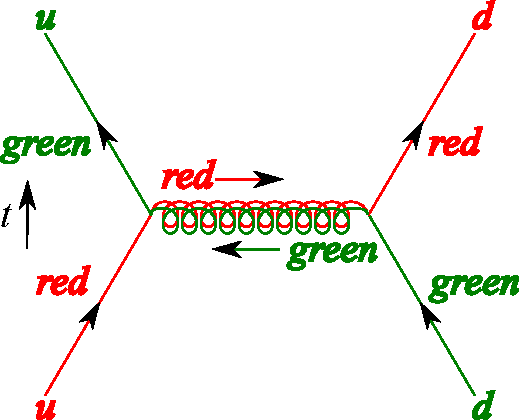
\includegraphics[scale=0.6]{qcd} % In qcd.svg as a layer
  \caption{Quark--gluón interaction}
  \label{fig:qcd}
\end{figure}
\end{frame}
Mientras que el segundo y tercer término dan lugar a autointeracciones de los gluones como se muestra en la Figura \ref{fig:qcd3gluon}
\begin{frame}
\begin{figure}
  \centering
  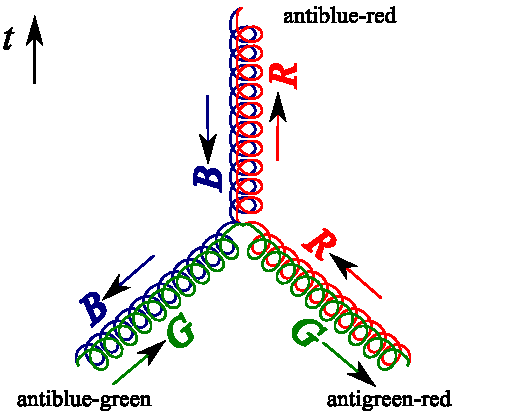
\includegraphics[scale=0.8]{qcd3gluon} 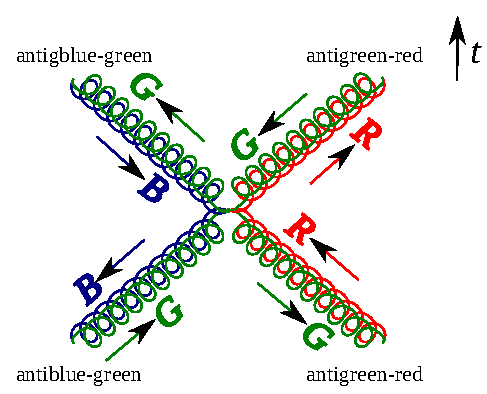
\includegraphics[scale=0.8]{qcd4} % In qcd.svg as a layer
  \caption{Triple--gluon and quartic--gluon self--interactions. The anticolors are the colors running back in time.}
  \label{fig:qcd3gluon}
\end{figure}
\end{frame}

Estás interacciones dan lugar a la estructura interna del protón mostrada en la figura~\ref{fig:prt}. Ver también \url{http://bit.ly/Baryon}

\begin{frame}
  \begin{figure}
    \centering
  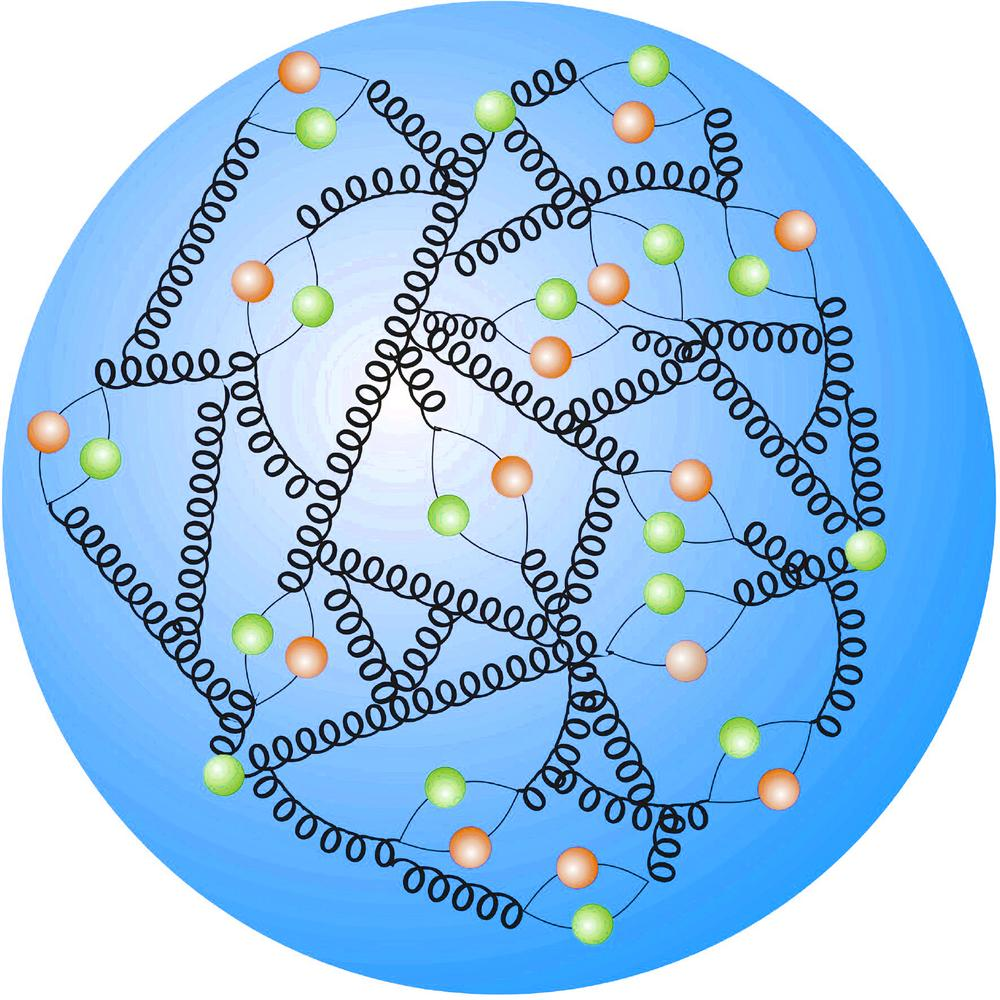
\includegraphics[scale=0.15]{proton}    
    \caption{En la esctructura interna del protón, además de los tres quarks de valencia representados en la figura como las tres partículas verdes aisladas, también están los gluones y los pares quark-antiquark. Estos últimos representados como las partículas naranja. Fuente: \href{http://www.desy.de/news/news_search/index_eng.html?openDirectAnchor=829}{desy.de}}
    \label{fig:prt}
  \end{figure}

\end{frame}

Todas las interacciones están determinadas en términos de una única constante de acoplamiento $g_s$. Las autointeracciones gauge pueden explicar aspectos de la interacción fuerte como la libertada asintótica, que consiste en que las interacciones fuertes se vuelven más débiles a distancias cortas. 

En términos de índices de color la corriente, y las otras partes del Lagrangiano, pueden escribirse como
\begin{equation}
  \label{eq:223qft}
  J^\mu_a=-g_s\bar{q}^\alpha\gamma^\mu q^\beta\left(\frac{\lambda_a}{2}\right)_{\alpha\beta}.
\end{equation}
Note que tanto para la Electrodinámica Cuántica como para la Cromodinámica Cuántica la corriente $\bar{\psi}\Gamma\psi$ es vectorial. Para las interacciones débiles la estructura es más complicada y requiere un conocimiento más profundo de la ecuación de Dirac y sus soluciones.


\subsection{Ecuaciones de Euler--Lagrange}
\label{sec:ecuaciones-de-euler-1}
Sigiendo los mismos procedimientos anteriores debemos llegar a los siguientes resultados. Para el campo $\Psi$ tememos
\begin{align}
  \underbrace{(i\gamma^\mu\mathcal{D}_\mu-m)}_{3\times 3 }\underbrace{\Psi}_{3\times 1}=0\,,
\end{align}
correspondientes a 3 ecuaciones, una para cada color.

En el caso del campo gauge $G_{\mu}^{a}$, tenemos
\begin{align}
  &\partial_\mu\left[\frac{\partial\mathcal{L}}{\partial\left(\partial_\mu G_\nu^a\right)}\right]-\frac{\partial\mathcal{L}}{\partial G_\nu^a}\nonumber\\
=&\partial_\mu\left\{-  \widetilde{G}^{\mu\nu}_a-\frac{1}{2}g_s f_{dbc}G_b^\rho G^\sigma_c\frac{\partial}{\partial\left(\partial_\mu G_\nu^a\right)}
\left(\partial_\rho G_\sigma^d-\partial_\sigma G_\rho^d\right)\right\}
-g_s\overline{\Psi}\gamma^\nu\frac{\lambda_a}{2}\Psi\nonumber\\
&+\frac{g_s}{2} f^{dbc}\widetilde{G}^{\rho\sigma}_d(\delta_{\rho\nu}\delta_{ba}G^c_\sigma+G^b_\rho\delta_{\sigma\nu}\delta_{ca})
+\frac{g_s}{4}f^{ibc}f_{ide}(g^{\rho\alpha}g^{\sigma\beta}G^b_{\alpha}G^c_\beta G^d_\rho G^e_\sigma)\nonumber\\
  =&\partial_\mu\left\{- \widetilde{G}^{\mu\nu}_a-\frac{1}{2}g_s f_{dbc}G_b^\rho G^\sigma_c
\left(\delta_{\rho\mu}\delta_{\sigma\nu}\delta_{da}-\delta_{\sigma\mu}\delta_{\rho\nu}\delta_{da}\right)\right\}
-g_s\overline{\Psi}\gamma^\nu\frac{\lambda_a}{2}\Psi\nonumber\\
&+\frac{g_s}{2} f^{dac}\widetilde{G}^{\nu\sigma}_dG^c_\sigma
+\frac{g_s}{2} f^{dba}\widetilde{G}^{\rho\nu}_dG^b_\rho\nonumber\\
&+\frac{g_s}{4}f^{ibc}f_{ide}g^{\rho\alpha}g^{\sigma\beta}(\delta_{\alpha\nu}\delta_{ba}G^c_\beta G^d_\rho G^e_\sigma+G^b_{\alpha}\delta_{\beta\nu}\delta_{ca}G^d_\rho G^e_\sigma+G^b_{\alpha}G^c_\beta\delta_{\rho\nu}\delta_{da}G^e_\sigma+G^b_{\alpha}G^c_\beta G^d_\rho\delta_{\sigma\nu}\delta_{ea})\nonumber\\
  =&-\partial_\mu\left\{  \widetilde{G}^{\mu\nu}_a-\frac{1}{2}g_s f^{abc}G_b^\mu G^\nu_c
+\frac{1}{2}g_s f_{abc}G_b^\nu G^\mu_c\right\}
-g_s\overline{\Psi}\gamma^\nu\frac{\lambda_a}{2}\Psi\nonumber\\
&-\frac{g_s}{2} f^{adc}\widetilde{G}^{\nu\sigma}_dG^c_\sigma
-\frac{g_s}{2} f^{adb}\widetilde{G}^{\nu\rho}_dG^b_\rho\nonumber\\
&+\frac{g_s}{4}f^{iac}f_{ide}g^{\rho\nu}g^{\sigma\beta}G^c_\beta G^d_\rho G^e_\sigma
+\frac{g_s}{4}f^{iba}f_{ide}g^{\rho\alpha}g^{\sigma\nu}G^b_{\alpha}G^d_\rho G^e_\sigma
+\frac{g_s}{4}f^{ibc}f_{iae}g^{\nu\alpha}g^{\sigma\beta}G^b_{\alpha}G^c_\beta G^e_\sigma\nonumber\\
&+\frac{g_s}{4}f^{ibc}f_{ida}g^{\rho\alpha}g^{\nu\beta}G^b_{\alpha}G^c_\beta G^d_\rho\,.
\end{align}
Desarrollando los cuatro últimos términos, tenemos

\begin{align}
  &\frac{g_s}{4}f^{iac}f_{ide}g^{\rho\nu}g^{\sigma\beta}G^c_\beta G^d_\rho G^e_\sigma
+\frac{g_s}{4}f^{iba}f_{ide}g^{\rho\alpha}g^{\sigma\nu}G^b_{\alpha}G^d_\rho G^e_\sigma
+\frac{g_s}{4}f^{ibc}f_{iae}g^{\nu\alpha}g^{\sigma\beta}G^b_{\alpha}G^c_\beta G^e_\sigma\nonumber\\
&+\frac{g_s}{4}f^{ibc}f_{ida}g^{\rho\alpha}g^{\nu\beta}G^b_{\alpha}G^c_\beta G^d_\rho\nonumber\\
=&\frac{g_s}{4}f^{iac}f_{ide}G_d^\nu G_c^\mu G^e_\mu
+\frac{g_s}{4}f^{iba}f_{ide}G_e^\nu G_b^{\mu}G^d_\mu
+\frac{g_s}{4}f^{ibc}f_{iae}G_b^{\nu}G_c^\mu G^e_\mu
+\frac{g_s}{4}f^{ibc}f_{ida}G_c^\nu G_b^{\mu}G^d_\mu\nonumber\\
=&  \frac{g_s}{4}f^{dac}f_{dje}G_j^\nu G_c^\mu G^e_\mu
+\frac{g_s}{4}f^{dca}f_{dje}G_e^\nu G_c^{\mu}G^j_\mu
+\frac{g_s}{4}f^{dbc}f_{dae}G_b^{\nu}G_c^\mu G^e_\mu
+\frac{g_s}{4}f^{dbc}f_{dea}G_c^\nu G_b^{\mu}G^e_\mu\nonumber\\
=&  \frac{g_s}{4}f^{dac}f_{dje}G_j^\nu G_c^\mu G^e_\mu
+\frac{g_s}{4}f^{dca}f_{dje}G_e^\nu G_c^{\mu}G^j_\mu
+\frac{g_s}{4}f_{dac}f^{dje}G_j^{\nu}Gc_e^\mu G^c_\mu
+\frac{g_s}{4}f_{dca}f^{dje}G_e^\nu G_j^{\mu}G^c_\mu\nonumber\\
=&  -\frac{g_s}{4}f^{abc}G^b_\mu f_{cej}G_e^\mu G_j^\nu
-\frac{g_s}{4}f^{abc}G^b_{\mu}f_{cej}G_e^\mu G_j^\nu
-\frac{g_s}{4}f_{abc}G^b_\mu f^{cej}G_e^\mu G_j^{\nu}
-\frac{g_s}{4}f_{abc}G^b_\mu f^{cej}G_e^{\mu}G_j^\nu\nonumber\\
=&-g_sf_{abc}G^b_\mu f^{cej}G_e^{\mu}G_j^\nu
\end{align}
Entonces
\begin{align}
    &\partial_\mu\left[\frac{\partial\mathcal{L}}{\partial\left(\partial_\mu G_\nu^a\right)}\right]-\frac{\partial\mathcal{L}}{\partial G_\nu^a}\nonumber\\
    =&\partial_\mu\left(-  \widetilde{G}^{\mu\nu}_a-g_s f^{abc}G_b^\mu G^\nu_c
\right)
-g_s\overline{\Psi}\gamma^\nu\frac{\lambda_a}{2}\Psi
-g_s f^{acd}G^c_\mu\widetilde{G}^{\mu\nu}_d
-g_sf_{acd}G^c_\mu f^{dej}G_e^{\mu}G_j^\nu\nonumber\\
      =&-\partial_\mu{G}^{\mu\nu}_a-g_s f^{acd}G^c_\mu{G}^{\mu\nu}_d
-g_s\overline{\Psi}\gamma^\nu\frac{\lambda_a}{2}\Psi=0\,.
\end{align}
Por lo tanto, las ecuaciones de Euler--Lagrange para $G_\nu^a$, son
\begin{align}
\label{eq:Gmuael}
\partial_\mu{G}^{\mu\nu}_a+g_s f^{acd}G^c_\mu{G}^{\mu\nu}_d
=-g_s\overline{\Psi}\gamma^\nu\frac{\lambda_a}{2}\Psi\,.
\end{align}
\begin{align}
\label{eq:Gmuael}
\partial_\mu{G}^{\mu\nu}_a-i g_s i f^{acd}G^c_\mu{G}^{\mu\nu}_d
=&-g_s\overline{\Psi}\gamma^\nu\frac{\lambda_a}{2}\Psi\nonumber\\
\delta^a_d\partial_\mu{G}^{\mu\nu d}-i g_s \left(-i f^{cad}\right)G^c_\mu{G}^{\mu\nu}_d
=&-g_s\overline{\Psi}\gamma^\nu\frac{\lambda_a}{2}\Psi\Psi\nonumber\\
\delta^a_d\partial_\mu{G}^{\mu\nu d}-i g_s {\left[\widetilde{\Lambda_c}\right]^a}_d G^c_\mu{G}^{\mu\nu d}
=&-g_s\overline{\Psi}\gamma^\nu\frac{\lambda_a}{2}\Psi\Psi\nonumber\\
{\left[ \mathcal{D}_\mu \right]^a}_d{G}^{\mu\nu d}
=&-g_s\overline{\Psi}\gamma^\nu\Lambda^{a}\Psi \nonumber\\
  \mathcal{D}_\mu{\boldsymbol{G}}^{\mu\nu}
=&-g_s\overline{\Psi}\gamma^\nu\boldsymbol{\Lambda}\Psi\,.
\end{align}
\begin{frame}[fragile,allowframebreaks]
por lo tanto
\begin{align}
  \mathcal{D}_\mu{\boldsymbol{G}}^{\mu\nu}
=&-g_s\overline{\Psi}\gamma^\nu\boldsymbol{\Lambda}\Psi\,,
\end{align}
donde $\boldsymbol{G}^{\mu\nu}$ y $\boldsymbol{\Lambda}$ son vectores en el espacio $SU(3)$. 
Además, hemos definido la derivada covariante en la representación adjunta como matrix  $8\times8$ 
\begin{align}
  \mathcal{D}_{\mu}=\mathbf{1}\partial_{\mu}-i g_s \widetilde{\Lambda}_a G_{\mu}^{a} 
\end{align}
Tenemos entonces 4 ecuaciones tipo ecuaciones Maxwell para cada gluón, $G_{\mu}^{a}$, por lo que en total
hay 32 ecuaciones tipo Maxwell acopladas.

La ec.\eqref{eq:Gmuael} puede reescribirse como:
\begin{align}
  \partial_\mu G^{\mu\nu}_a=-g_s\left[{\color{red}f_{abc}G^b_\mu G^{\mu\nu}_c}+\bar{\Psi}\gamma^\nu\frac{\lambda_a}{2}\Psi  \right]
\end{align}
\end{frame}
y usando el hecho que $\partial_\mu\partial_\nu=\partial_\nu\partial_\mu$:
\begin{align}
  \partial_\nu\partial_\mu G^{\mu\nu}_a=&\partial_\nu\partial_\mu\widetilde{G}^{\mu\nu}+g_s\partial_\nu\partial_\mu\left(f_{abc}G^\mu_bG^\nu_c\right)\nonumber\\
=&0+\frac{1}{2}\left[g_s\partial_\nu\partial_\mu\left(f_{abc}G^\mu_bG^\nu_b\right)+g_s\partial_\nu\partial_\mu\left(f_{abc}G^\mu_bG^\nu_c\right)\right]\nonumber\\
=&\frac{1}{2}\left[g_s\partial_\nu\partial_\mu\left(f_{abc}G^\mu_bG^\nu_b\right)+g_s\partial_\mu\partial_\nu\left(f_{abc}G^\mu_bG^\nu_c\right)\right]\nonumber\\
=&\frac{1}{2}\left[g_s\partial_\nu\partial_\mu\left(f_{abc}G^\mu_bG^\nu_b\right)+g_s\partial_\nu\partial_\mu\left(f_{acb}G^\nu_cG^\mu_b\right)\right]\nonumber\\
=&\frac{1}{2}\left[g_s\partial_\nu\partial_\mu\left(f_{abc}G^\mu_bG^\nu_b\right)-g_s\partial_\mu\partial_\nu\left(f_{abc}G^\mu_bG^\nu_c\right)\right]\nonumber\\
=&0\,,
\end{align}
como en el caso Abeliano, tenemos la corriente
% conservada
% \begin{align}
%   \partial_\nu j^\nu=0\,,
% \end{align}
% donde
\begin{frame}[fragile,allowframebreaks]
\begin{align}
  \label{eq:noabeljnu}
j^{\nu}_{a}=-\frac{\partial\mathcal{L}}{\partial G_\nu^a}\,,
\end{align}
tal que
\begin{align}
\label{eq:jnuqcd}
  j^\nu_a=&g_s\left[f_{abc}G^b_\mu G^{\mu\nu}_c+\bar{\Psi}\gamma^\nu\frac{\lambda_a}{2}\Psi  \right]\,.
\end{align}

El primer término corresponde a las autointeracciones y el segundo a la corriente de color generada por los quarks.
\end{frame}

% De otro lado
% \begin{align}
%   \mathcal{D}_\mu{\boldsymbol{G}}^{\mu\nu}
% =&-g_s\overline{\Psi}\gamma^\nu\boldsymbol{\Lambda}\Psi\nonumber\\
% U\mathcal{D}_\mu U^\dagger U {\boldsymbol{G}}^{\mu\nu}
% =& -g_sU\overline{\Psi}\gamma^\nu\boldsymbol{\Lambda}\Psi\nonumber\\
% \mathcal{D}_\mu  U {\boldsymbol{G}}^{\mu\nu}
% =&-g_sU\overline{\Psi}\gamma^\nu\boldsymbol{\Lambda}\Psi\,,
% \end{align}
% y haciendo la expansión infinitesimal
% \begin{align}
% \mathcal{D}_\mu  (\boldsymbol{1}-i\Lambda_a \theta^a) {\boldsymbol{G}}^{\mu\nu}
% =&-g_s(\boldsymbol{1}-i\Lambda_a \theta^a)\overline{\Psi}\gamma^\nu\boldsymbol{\Lambda}\Psi \nonumber\\
% \mathcal{D}_\mu{G}^{\mu\nu a}  -i\Lambda_a {G}^{\mu\nu a} \theta^a
% =&-g_s\overline{\Psi}\gamma^\nu\Lambda^{a}\Psi -i\Lambda_a \theta^a\overline{\Psi}\gamma^\nu\Lambda^{a}\Psi\,,
% \end{align}
% e igualando coeficientes, tenemos
% \begin{align}
% \label{eq:matrixform}
%   \mathcal{D}_\mu{{G}}^{\mu\nu}
% =&-g_s\overline{\Psi}\gamma^\nu\boldsymbol{\Lambda}\Psi\,.
% \end{align}
\subsection{Corrientes conservadas}

\begin{align}
  \mathcal{E}_1 a_1 + \mathcal{E}_2 a_2 + \mathcal{E}_3 a_3=& \partial_{\mu} \left( \mathcal{E}_1 b_1^{\mu} + \mathcal{E}_2 b_2^{\mu} + \mathcal{E}_3 b_3^{\mu}   \right) \,.
\end{align}
Asumimos que la ecuaciones de Euler Lagrange para los fermiones se satisfacen (además $b_1^{\mu}=b_2^{\mu}=0$), entonces
\begin{align}
   \mathcal{E}_1 a_1 + \mathcal{E}_2 a_2 +  \mathcal{E}_3 a_3=& \partial_{\mu} \left(  \mathcal{E}_3 b_3^{\mu}   \right) \,.
\end{align}

Haciendo uso de la ec.~\eqref{eq:noabeljnu}
\begin{align}
  \partial_{\mu} \left(  \mathcal{E}_3 b_3^{\mu}   \right)=&
                                                \partial_{\mu} \left\{  \partial_\nu\left[\frac{\partial\mathcal{L}}{\partial\left(\partial_\nu G_\mu^a\right)}\right]-\frac{\partial\mathcal{L}}{\partial G_\mu^a}  \right\} \nonumber\\
  =&-\partial_{\mu}\left( \frac{\partial\mathcal{L}}{\partial G_\mu^a} \right) \nonumber\\
=& \partial_{\mu} j^{\mu}\,,
\end{align}
\begin{align}
  \left\{ \partial_{\mu}\left[{ \frac{\partial {\cal L}}{\partial \left( \partial_{\mu}\Psi \right)}}\right]-\frac{\partial{\cal L}}{\partial\Psi}  \right\}a_1+
  a_{2}\left\{ \partial_{\mu}\left[\cancel{ \frac{\partial {\cal L}}{\partial \left( \partial_{\mu}\overline{\Psi} \right)}}\right]-\frac{\partial{\cal L}}{\partial\overline{\Psi}}  \right\}+
  \left\{ \partial_\mu\left[\frac{\partial\mathcal{L}}{\partial\left(\partial_\mu G_\nu^a\right)}\right]-\frac{\partial\mathcal{L}}{\partial G_\nu^a} \right\} a_3 =&
 \partial_{\mu}j^{\mu}\nonumber\\
  \partial_{\mu}\left[ \frac{\partial {\cal L}}{\partial \left( \partial_{\mu}\Psi \right)}a_{1}+
  \frac{\partial\mathcal{L}}{\partial\left(\partial_\mu G_\nu^a\right)}a_{3}\right]
-\frac{\partial {\cal L}}{\partial \left( \partial_{\mu}\Psi \right)}\partial_{\mu} a_1
  -\frac{\partial{\cal L}}{\partial\Psi}a_{1}
  -a_2\frac{\partial{\cal L}}{\partial\overline{\Psi}}
  -\frac{\partial\mathcal{L}}{\partial\left(\partial_\mu G_\nu^a\right)}\partial_{\mu}a_{3}
  -\frac{\partial\mathcal{L}}{\partial G_\nu^a}a_{3}=&\partial_{\mu}j^{\mu}\,.
\end{align}
Ya que, usando $a_{3}=f_{a}^{bc} G^{\mu}_{c} $
%TODO: Demostrar...
\begin{align}
 \frac{\partial {\cal L}}{\partial \left( \partial_{\mu}\Psi \right)}\partial_{\mu} a_1
  +\frac{\partial{\cal L}}{\partial\Psi}a_{1}
  +a_{2}\frac{\partial{\cal L}}{\partial\overline{\Psi}}
  +\frac{\partial\mathcal{L}}{\partial\left(\partial_\mu G_\nu^a\right)}\partial_{\mu}a_{3}
  +\frac{\partial\mathcal{L}}{\partial G_\nu^a}a_{3}=0\,,
\end{align}
el Segundo Teorema de Noether establece que
\begin{align}
  j^{\mu}=\frac{\partial {\cal L}}{\partial \left( \partial_{\mu}\Psi \right)}a_{1}+
  \frac{\partial\mathcal{L}}{\partial\left(\partial_\mu G_\nu^a\right)}a_{3}\,.
\end{align}
% TODO: Demostrar que la formula es válida

\section{Anotaciones finales}


Hemos visto que bajo una simetría continu $\operatorname{U}(1)$
\begin{itemize}
 \item Un campo escalar real se convierte en un campo escalar complejo
\item Un campo vectorial se convierte en un campo tensorial
\item Un campo de Weyl se convierte en un campo de Dirac
\end{itemize}


% \begin{subappendices}
% \end{subappendices}


\section{Ejercicios}
\begin{enumerate}
\item Utilizando la forma más simétrica del Lagrangiano
Para analizar mejor las implicaciones de este teorema, es mejor tener una forma más simétrica del Lagrangiano de Dirac
\begin{align}
\mathcal{L}=\frac{i}{2}\overline{\psi} \gamma^\mu{\partial_{\mu}} \psi-\frac{i}{2}\left(\partial_{\mu} \overline{\psi}\right) \gamma^{\mu} \psi-m \overline{\psi} \psi-\frac{1}{4} F^{\mu \nu} F_{\mu \nu}\,,
\end{align}
cuya forma invariante gauge local se obtiene reemplazando la derivada normal por la derivada covariante
\begin{align}
\label{eq:silagqed}
\mathcal{L}=&\frac{i}{2}\overline{\psi} \gamma^\mu{\mathcal{D}_{\mu}} \psi-\frac{i}{2}\overline{\left(\mathcal{D}_{\mu} \psi\right)} \gamma^{\mu} \psi-m \overline{\psi} \psi-\frac{1}{4} F^{\mu \nu} F_{\mu \nu}\nonumber\\
=&\frac{i}{2}\overline{\psi} \gamma^\mu{\partial_{\mu}} \psi-\frac{i}{2}\partial_{\mu} \overline{\psi} \gamma^{\mu} \psi
+e \bar{\psi} \gamma^{\mu} \psi A_{\mu}
-m \overline{\psi} \psi-\frac{1}{4} F^{\mu \nu} F_{\mu \nu}\,.
\end{align}
establezca el segundo teorema de Noether
\begin{align}
  \sum_i \mathcal{E}_ia_i=&\sum_i  \partial_{\mu}   \left(  \mathcal{E}_i b^{\mu}_i  \right)\nonumber\\
  \mathcal{E}_1a_1+\mathcal{E}_2a_2=&
   \partial_{\mu}   \left(  \mathcal{E}_3 b^{\mu}_3  \right)\,.
\end{align}
\item Encuentre el Hamiltoniano para la QED
\end{enumerate}



\renewcommand{\labelenumi}{\theenumi} %noinstiki

% \left(\right)
%
%%% Local Variables: 
%%% mode: latex
%%% TeX-master: "fullnotes"
%%% ispell-local-dictionary: "castellano8"
%%% End: